% Nejprve uvedeme tridu dokumentu s volbami
\documentclass[bc,male,java,dept456]{diploma}						% jednostranny dokument

\usepackage[czech]{babel}
%\usepackage[cp1250]{inputenc}
\usepackage[utf8]{inputenc}
\usepackage{comment}
\usepackage{graphicx}
\usepackage{url}
\usepackage{longtable}
%\usepackage{dialogue}

%\usepackage[a-1b]{pdfx}


\begin{comment}
TODO
 - projít celou diplomku
 - zkontrolovat TODO
 - znovu projít chyby
 - znovu zkontrolovat přesahy


Projít si: \subsection{Webové aplikace}
 
DONE
 - přepsat Abstrakt
 - vyhledat " a a "
 - doplnit REFERENCE
 - všem tabulkám doplnit CAPTION
 - odkazovat na tabulky
 - fixnout přetékající text
 - dopsat ZHODNOCENÍ
 - dopnit názor chum.ly
 
Před tiskem:
 - ******************* upravit DATUM u podpisu *****************
 
Po tisku:
 - zkompilovat do PDFX-A
	
\end{comment}



\setcounter{secnumdepth}{2}

\begin{comment}

> Taky bych by opatrný s kombinací webová analytika…často je to ve větě i se slovy analytika a analýza, což působí divně, např. 	první věta v úvodu

> Všude musí být citovány zdroje a reference, např. Heatmapy, pokud jste je nedělal sám, pak není jasné, odkud jsou
> Pozor rozházené odstavce vůči ořezu, přesahy řádků
> Část věnující se vašemu řešení bych nenazíval Nový nástroj

> Pokuste se sjednotit vzhled obrázků a schémat
Pokusil, ještě projdu.

> V části 3 by mělo být více o tom, jak to řešíte..nejen z pohledu koncepčního (uživatelé), ale z pohledu procesního…třeba i nějaký diagram aktivit apod. Není tam jasná linka, od psecifikace požadavků k použití resp. implementaci


\end{comment}



% Zadame pozadovane vstupy pro generovani titulnich stran.
\Author{Michal Hantl}

\Title{Nástroj pro monitorování chování uživatelů webových aplikací}

\EnglishTitle{Tool for Behavior Monitoring of Web Applications Users}

\SubmissionDate{5. května 2011}

\PrintPublicationAgreement{true}



\Thanks{Rád bych na tomto místě poděkoval svým rodičům za podporu během celého studia, panu Ing. Michalovi Radeckému, za vedení během vypracování diplomové práce a své přítelkyni Míše za neskonalou toleranci, kterou mi v tomto životě projevuje.}





\CzechAbstract{Tato diplomová práce se zabývá problematikou webové analytiky, novou metodou měření uživatelské interakce s webem a nástrojem pro analýzu webových aplikací. Úvodem nastiňuje nové výzvy we webové analytice. V kapitole Webová analytika popisuje historii sběru a vyhodnocování dat na webu a současné způsoby sběru a interpretace dat. Kapitola Analýza webových aplikací se zaměřuje na webové aplikace z pohledu nové metody sběru a interpretace dat. Kapitola Technické řešení se popisuje detaily zpracování dat a využívané technologie. Případová studie se věnuje nasazení nástroje do provozu na platformě Google AppEngine a zhodnocuje výsledky.
}

\CzechKeywords{webová analytika, chování uživatelů, webová aplikace, diplomová práce}

\EnglishAbstract{This thesis is concerned with web analytics, new method of measuring user interaction with the web and with a tool for web application analysis. Chapter one outlines new challenges in web analytics. Chapter two describes history of web analytics' data gathering and interpretation. Chapter three is focused on web applications from the point of new way of gathering and data interpretation. Chapter four describes the details of data processing and technologies involved. In fifth chapter, the created tool is deployed on Google AppEngine and used in production application and then conclusions are drawn.
}

\EnglishKeywords{web analytics, user behaviour, web application, master thesis}





% Pridame pouzivane zkratky (pokud nejake pouzivame).
\AddAcronym{CDN}{Síť pro doručování obsahu (Content Delivery Network)}
\AddAcronym{GUI}{Grafické uživatelské rozhraní (Graphical User Interface)}
\AddAcronym{HTML}{Jazyk pro vytváření webových stránek (HyperText Markup Language)}
\AddAcronym{HTTP}{Hypertextový protokol (Hypertext Transfer Protocol)}
\AddAcronym{PPC}{Platba za proklik (Pay per click)}
\AddAcronym{ROI}{Zisk z investice (Return on Investment)}






% Zacatek dokumentu
\begin{document}

% Nechame vysazet titulni strany.
\MakeTitlePages

% Asi urcite budeme potrebovat obsah prace.
\tableofcontents
\cleardoublepage	% odstrankujeme, u jednostranneho dokumentu o jednu stranku, u oboustrenneho o dve

% Jsou v praci tabulky? Pokud ano vysazime jejich seznam.
% Pokud ne smazeme nasledujici makro.
\listoftables
\cleardoublepage	% odstrankujeme, u jednostranneho dokumentu o jednu stranku, u oboustrenneho o dve

% Jsou v praci obrazky? Pokud ano vysazime jejich seznam.
\listoffigures
\cleardoublepage	% odstrankujeme, u jednostranneho dokumentu o jednu stranku, u oboustrenneho o dve


% Jsou v praci vypisy programu? Pokud ano vysazime jejich seznam.
\lstlistoflistings
\cleardoublepage	% odstrankujeme, u jednostranneho dokumentu o jednu stranku, u oboustrenneho o dve










\section{Úvod}
\label{sec:Uvod}


Tato diplomová práce se zabývá webovou analytikou a novým nástrojem pro analytiku webových aplikací. 

Od vzniku webových stránek se web rozvíjel až do dnešní podoby a webová analytika\cite{kaushik} ho provázela. Čím sofistikovanějšími se webové stránky stávaly, tím důmyslnější způsoby byly nacházeny k analýze uživatelského chování.

Zpočátku byly používány nástroje na straně serveru, které pasivně analyzovaly data o návštěvách stránek. V polovině devadesátých let masivní vývoj webových prohlížečů přesunul sběr dat na stranu klienta, kde umožnil aktivní sběr dat o uživatelském chování.

Sběr dat na straně klienta umožnil rozvoj jednoduše použitelných nástrojů pro webovou analytiku. Odpadla nutnost instalovat nástroj na server, stačilo vložit skript na stránky. Tyto nástroje však stále kopírují konvenční přístup k analýze návštěvníků.

Současné metody měření a interpretace dat dobře vyhovují jednorázovým účelům, jako je měření konverze reklamní kampaně, nebo poskytují statistiky, jako je top 10 nejnavštěvovanějších stránek na serveru v daném období. Objevují se však již nástroje, které se snaží poskytnout něco navíc.

Kromě webových stránek jsou na internetu také webové aplikace. Díky moderních technologiích jako HTML5 se začíná smazávat rozdíl mezi možnostmi desktopových aplikací a webových. Tento trend potvrzuje i to, že Google připravuje svůj vlastní operační systém Chrome OS\footnote{\url{http://www.google.com/chromeos/}}, který je výhradně založen na webovém prohlížeči.

Možnosti webových aplikací jsou již nyní rozšířeny o podporu audia, videa (včetně manipulace) a zobrazení trojrozměrných objektů pomocí technologie WebGl\cite{webgl}. Někteří i tak budou tvrdit, že webové aplikace se nikdy nebudou moci měřit s desktopovými. Na druhou stranu dnes již existují pluginy do prohlížečů, které jakoby umožňují spouštět nativní kód jako SilverLight, nebo Flash a skutečnou podporu nativního kódu slibuje například technologie Native Client, kterou prosazuje Google ve svém prohlížeči Chrome.

Můžeme tedy očekávat nárůst počtu webových a\-pli\-ka\-cí, které nezaostávají za desktopovými. 


\subsection{Cíl práce}

Cílem práce je vytvoření nástroje, jakožto podpory pro aplikaci a navržení metody zí\-ská\-vá\-ní informací o chování uživatele webové aplikace. Nebude se jednat pouze o klasický přístup založený na sběru statistických dat anonymních návštěvníků, ale o využití znalosti o konkrétním uživateli, jeho chování, využívání funkcí a služeb webové aplikace.

\begin{itemize}
	\item Zanalyzujte a popište možnosti monitorování chování návštěvníků webových strá\-nek a aplikací, a to s důrazem na získané informace a metody jejich zpracování.
	\item Navrhněte a popište technické postupy a metody pro získávání potřebných informací a dat o chování uživatele.
	\item Naimplementujte nástroj pro monitorování chování návštěvníků webových aplikací, a to včetně modulu pro integraci do jakékoli webové (HTML) aplikace.
	\item Vyvinutý nástroj aplikujte do provozu a získaná data analyzujte a popište závěry plynoucí ze získaných informací.
	\item Zhodnoťte vyvinutý nástroj především z pohledu reálného nasazení a jeho přínosů, porovnejte jej s obdobnými nástroji a jejich metodami.
\end{itemize}





\section{Webová analytika}

Tato kapitola popisuje vznik webové analytiky a způsoby sběru a interpretace dat v obecné rovině. 



\subsection{Historie}


Dnešní nástroje v podstatě kopírují způsob interpretace dat a proto je vhodné nastínit historii webové analytiky.

Na začátku devadesátých let došlo ke zrození WWW stránek. Uživatelé tehdy pro\-hlí\-želi statické stránky a pokaždé, když si nějakou prohlédli, vznikl záznam v logovacím souboru, takzvaný "hit". A počet hitů se stal ukazatelem úspěšnosti webový stránek.

\bigskip

\begin{lstlisting}[label=src:Plain,caption=Ukázka záznamu z logovacího souboru]
10.20.30.40 - - [26/Apr/2000:00:23:48 -0400] "GET /index.html HTTP/1.0" 200 6248 "http://www.jafsoft.com/asctortf/" "Mozilla/4.05 (Macintosh; I; PPC)"
10.20.30.40 - - [26/Apr/2000:00:23:48 -0400] "GET /background.gif HTTP/1.0" 200 4005 "http://www.example.org/" "Mozilla/4.05 (Macintosh; I; PPC)"
\end{lstlisting}

\bigskip

Logovací soubor obsahuje jeden řádek pro každou návštěvu stránky, nebo souboru na serveru. Nástroj pro analýzu logovacích souborů z toho pak dokáže zjistit kolik měl server návštěv každý den, z kolika unikátních IP adres, které stránky jsou nej\-na\-vště\-vo\-va\-něj\-ší a kolik bylo přenesených dat.

V roce devadesát čtyři vznikl grafický webový prohlížeč s názvem Mosaic. Díky jeho snadné instalaci a srozumitelnému uživatelskému rozhraní se web otevřel široké veřejnosti. Tento prohlížeč byl později přejmenován na Netscape a v roce 1995 ho po\-u\-ží\-va\-lo 80\% uživatelů internetu.

V roce devadesát pět vznikl Analog - nástroj pro analýzu logovacích souborů. Jeho autor Stephen Turner ho poskytoval zdarma jako freeware pro několik platforem. Jednalo se o první sofistikovanější nástroj pro analýzu a zobrazení návštěvnosti webových stránek. V tabulce \ref{table:analog_output} je znázorněno, jak vypadal jeden z prvních textových výstupů programu analog.

\begin{table}[h]
	\centering	
\begin{tabular}{p{2cm} p{3cm} p{2cm} p{5cm}}
den&požadavků&stránek&\\
\hline
Pondělí			& 2012965			& 626	& ========= \\
Úterý			& 2490837			& 788	& ========== \\
Středa			& 3193776			& 880	& =========== \\
Čtvrtek			& 3188571			& 941	& ============= \\
Pátek			& 3589076			& 1076	& ===============\\
Sobota			& 3589076			& 1007	& ============= \\
Neděle			& 3036246			& 1261	& ======================\\
\end{tabular}



\begin{comment}
The data collection became unusable with the advent of search engines and their robots, proxies servers to surf anonymously, allocation of dynamic IP addresses by ISPs and cached content techniques. All these developments have rendered the use of log files inappropriate to analyze user behavior. The data contained in log files were indeed biased and unique visitor identification almost impossible. 
\end{comment}

\begin{comment}
\begin{figure}[h]
	\centering
	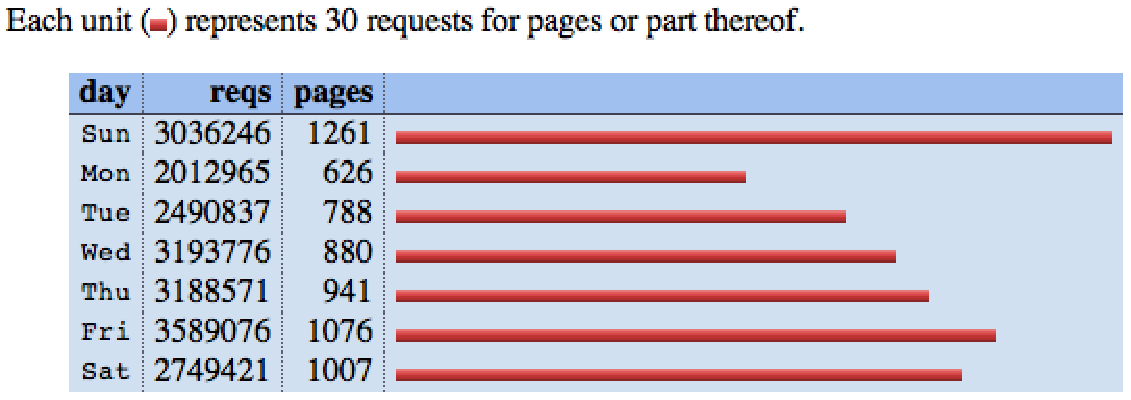
\includegraphics[width=14cm]{img/analog_daily.pdf}
	\caption{Analog - denní návštěvnost}
	\label{tab:analog_daily}
\end{figure}
\end{comment}





	\caption{Výpis návštěvnosti z programu Analog} 
	\label{table:analog_output}
\end{table}

V roce 1996 byl v obou nejpoužívanějších prohlížečích\cite{browser_market_share} k dispozici JavaScript. Tvůrce webových stránek na každou stránku umístil kód, který mu vygeneroval poskytovatel měřícího nástroje. 

Tento postup se zásadně liší od analýzy logových souborů. Místo statické analýzy zaznamenaných dat na straně serveru tento přístup data dynamicky sbírá na straně klienta.

Průlom v prohlížečích umožnil použití třetích stran pro sběr i vyhodnocení dat a tak dal vzniknout prvním online nástrojům pro webovou analytiku. V různých obměnách se tato technika používá dodnes.

V roce 2005 koupila\cite{urchin} společnost Google analytický systém Urchin on Demand a ještě v témž roce ho poskytla zdarma široké veřejnosti jako webovou aplikaci pod názvem Google Analytics. Pro obrovský zájem byl tento produkt zpřístupněn pouze omezenému počtu uživatelů. Od října roku 2006 byly znovu otevřeny volné registrace a dodnes se jedná o nejpoužívanější systém pro webovou analytiku.

S nástupem sociálních médií a chytrých mobilních zařízení dochází k nárůstu času, který uživatelé tráví na internetu. Poměrně k tomuto nárůstu se zvyšují investice do internetových stránek a webových aplikací. 

Na jedné straně je snaha dostat nové uživatele na svou stránku, to se dociluje na\-pří\-klad pomocí optimalizace pro vyhledávače, reklamních bannerů, nebo PPC reklamy\footnote{PPC - Pay per click, platba za proklik.}. V ta\-ko\-vém případě slouží webová analytika k měření efektivity jednotlivých kampaní a k jejich následné optimalizaci.

Na druhé je snaha pracovat s uživateli, které už webová stránka, nebo aplikace má. Zde je snaha identifikovat problémy a optimalizovat uživatelskou zkušenost. V obou případech je to webová analytika, která nám umožňuje získat přehled, optimalizovat a vyhodnotit návratnost investic.










\subsection{Sběr dat}

Podstatou webové analytiky je sběr a interpretace dat. Ten se za dobu existence webu vyvinul z pasivní formy analýzy logovacích souborů na serveru do dnešní - aktivního sběru dat na straně uživatele třetí stranou.

Tato podkapitola popisuje popisuje používané způsoby sběru dat s důrazem na to, jaké informace z nich získáváme, jaké další informace z nich můžeme vyčíst a jaké způ\-so\-by vizualizace se běžně vyskytují.



\subsubsection{Analýza dat z logovacích souborů}

Webové servery zaznamenávají zobrazení stránek do takzvaných logovacích souborů. Jedná se o soubory, ve kterých každý řádek představuje záznam o jednom zobrazení stránky, nebo například obrázku.

Když na začátku devadesátých let vznikl web, provozovatelé serverů si uvědomili, že tyto soubory umožňují získat informace o popularitě jejich stránek a tak začali měřit počet zobrazení, takzvaných "hitů". V té době se vyskytovaly většinou pouze dlouhé stránky bez obrázků nebo odkazů, takže počet zobrazení postačoval potřebám provozovatelů.

\bigskip

\begin{lstlisting}[label=src:logfile_record,caption=Formát logovacího souboru]
127.0.0.1 - frank [10/Oct/2000:13:55:36 -0700] "GET /apache_pb.gif HTTP/1.0" 200 2326
\end{lstlisting}

\bigskip

Výpis \ref{src:logfile_record} je ukázkou záznamu v logovacím souboru. Později docházelo k rozšíření tohoto formátu\cite{clf}, aby obsahoval další zajímavé informace, které mohl analytický sofwtare zpracovávat. Význam jednotlivých částí typického řádku logovacího souboru jsou po\-psá\-ny v tabulce \ref{tab:http_log_info}.

\begin{table}
	\centering      
	\begin{tabular}{ lp{9cm} }
  \verb!127.0.0.1! & IP adresa návštěvníka. Počet unikátních IP adres byl původně používán jako hrubý odhad počtu uživatelů. \\ \bigskip
  \verb!-! & pomlčka \\ \bigskip
  \verb!frank! & Uživatelské jméno. Tento údaj je přítomen v případě se stránka používá HTTP autentizaci. To platí pro stránky s omezením přístupu pro uzavřenou skupinu lidí a tudíž u náhodného návštěvníka stránky tento údaj nenajdeme. V takovém případě se místo uživatelského jména zaznamená pomlčka. \\ \bigskip
  \verb!10/Oct/2000! & Datum návštěvy. \\ \bigskip
  \verb!13:55:36! & Čas návštěvy, vztahuje se k časové zóně na serveru. \\ \bigskip  
  
  \verb!-0700! & Časová zóna. \\ \bigskip
  \verb!GET /apache_pb.gif! & Požadavek a verze HTTP protokolu \\ \bigskip
  \verb!HTTP/1.0! & Požadavek HTTP protokolu. GET je základním požadavkem, který signalizuje, že uživatel požaduje nějaký obsah. Další používaný požadavek je například POST, který se používá pro odeslání formuláře na server.  \\ \bigskip
  
  \verb!200! & Kód odpovědi. Kód 200 znamená vše v pořádku. Obvyklé a pro webovou analytiku také zajímavé jsou 404 - stránka nenalezena, 500 - problém na serveru, nebo 303 - přesměrování stránky. \\ \bigskip
  \verb!2326! & Délka odpovědi v bajtech. Sledování této veličiny spolu s počtem návštěv umožňuje identifikovat, který obsah nejvíce zatěžuje internetové připojení daného serveru.
	\end{tabular}
	\caption{Informace obsažené v HTTP hlavičce}
	\label{tab:http_log_info}
\end{table}






Jak web rostl, zvětšovala se i jeho složitost. Z jednoduchých stránek bez obrázků se staly různě provázené stránky s odkazy a obrázky. Stehně tak i nástroje pro analýzu logovacích souborů se stávaly sofistikovanějšími a začaly na sebe nabalovat další možnosti. Pole zaznamenávaných dat sbíraných v logovacích souborech byl rozšířen o další informace HTTP protokolu, kterými se zabývá další část kapitoly.





  
\subsection{Informace získané pomocí HTTP protokolu}

Prohlížení webových stránek na internetu je zajišťěno pomocí HTTP protokolu. HTTP je zkratka pro Hyper Text Tranfer Protokol, neboli protokol pro výměnu hypertextů (hypertextových stránek). Je to způsob jak webový prohlížeč komunikuje s webovým serverem.

Pomocí HTTP protokolu poskytuje prohlížeč informace o uživateli tak, aby webový server mohl co nejlépe vyhovět požadavku.

Formátem HTTP protokolu se na tomto nebudeme hlboce zabývat. Stačí vědět, že obsahuje podstatné jsou informace, které se používají ve webové analytice. Pro zajímavost je uveden příklad HTTP požadavku a některých základních informací, které obsahuje.

\bigskip

\begin{lstlisting}[label=src:Plain,caption=Ukázka HTTP požadavku]
GET /dumprequest HTTP/1.1
Host: djce.org.uk
Connection: keep-alive
Accept: application/xml,application/xhtml+xml,text/html;q=0.9,text/plain;q=0.8,image/png,*/*;q=0.5
User-Agent: Mozilla/5.0 (X11; U; Linux i686; en-US) AppleWebKit/534.16 (KHTML, like Gecko) Chrome/10.0.634.0 Safari/534.16
Accept-Encoding: gzip,deflate,sdch
Accept-Language: cs-CZ,cs;q=0.8
Accept-Charset: windows-1250,utf-8;q=0.7,*;q=0.3
\end{lstlisting}

Z hlaviček HTTP protokolů je možno získat většinu informací, se kterými analytické nástroje pracují. Následující text popisuje které jsou ty základní a jak se používají.

\subsubsection{Požadovaná stránka}

Zaznamenáváním, kolikrát je každá stránka vyžadována získáme počet zobrazení stránek na serveru. Tento údaj se v nejjednodušším příkladě používá k určení popularity jednotlivých stránek na webovém serveru. Z hlediska toho, jak jsou dnešní webové stránky strukturovány, dá se předpokládat, že čím hlouběji je stránka zanořená ve stromové struktuře webu, tím toto číslo bude menší. Například:

\begin{lstlisting}[label=src:Plain,caption=Distribuce návštěv ve stromové struktuře]
--+ Hlavni stranka 				(150x)
  |--+ Podstranka 1				( 50x)
  |  \-- Pod-pod stranka	( 10x)
  \--- Podstranka 2				( 50x)
\end{lstlisting}

Tato informace má různý význam v různých kontextech. Uvažujme informační server na kterém každý den vyjde několik článků v různých kategoriích. Hlavní stránka klade největší důraz na nejnovější články a v postranním panelu obsahuje odkazy na jednotlivé kategorie článků.

\begin{lstlisting}[label=src:Plain,caption=Struktura informačního serveru]
--+ Hlavni stranka
  |-- 1. Clanek A
  |-- 2. Clanek	B	
  |-- 3. Clanek	C
  ...
  |-- Kategorie clanku 1
  \-- Kategorie clanku 2
\end{lstlisting}

Pro kategorie znamená počet zobrazení popularitu jednotlivých kategorií. Tento údaj by měl být odpovídat počtu zobrazení článků v jednotlivých kategoriích a měl by se porovnávat k počtu zobrazení dalších kategorií. Například v případě že poměr návštěv kategorie vaření je velký ale poměr přečtení článků o vaření je malý, může to například znamenat, že kategorie je zajímavá ale neobsahuje tak zajímavé články.

Pro stránku, která představuje článek je počet zobrazení ukazatelem toho, jak je článek populární. S touto informaci je se dále pracuje a interpretuje se. Je třeba dát do kontextu:
\begin{itemize}
  \item{které webové stránky na daný článek odkázaly}
  \item{kolik vzniklo ke článku komentářů}
  \item{kolik lidí kliklo na článek z hlavní stránky}
  \item{jaký je u článku titulek a obrázek, jestli článek}
\end{itemize}


V kontextu webové aplikace se může jednat o údaj, který udává nejpoužívanější sadu funkcí. Následující příklad toto demonstruje na zjednodušené administraci E-shopu.

\begin{lstlisting}[label=src:Plain,caption=Struktura administrace elektronického obchodu]
--+ Administrace
  |-+ Objednavky
  | |-- nevyrizene
  | |-- vyrizene
  | \-- hledat
  |-- Zbozi
  \-- Nastaveni
\end{lstlisting}

V této fiktivní administraci E-shopu jsou tři hlavní podstránky - Objednávky, Zboží a Nastavení. V tomto případě počet zobrazení jednotlivých kategorií umožňuje zjistit (zhruba), jak často je pracováno s objednávkami v poměru se zbožím a nastavením.

V každém případu počet zobrazených stránek představuje trochu jinou informaci a je třeba je interpretovat v podle typu měřené stránky (případně aplikace) a toho jak ji uživatelé používají.

\subsubsection{Referrer}

Údaj refferer je stránka, ze které uživatel přišel. Dá se tedy zjistit, odkud uživatelé na stránku přicházejí a spočítat nejčastější zdroje návštěv.

Ještě zajímavější využití této informace je v případě, že uživatel přišel z vyhledávače. Pak se dá z referreru zjistit, jakou frázi uživatel vyhledával a jaké vyhledávače dominují v počtu přivedených zákazníků.

\subsubsection{Query string}

V query string části adresy se nacházejí údaje, které modifikují obsah stránky. V začátcích webů se takto odlišovaly dynamické stránky od statických. Je to část adresy stránky za otazníkem a často nese zajímavé informace. Například pokud zadáte "web analytics" do hledání v Google, bude adresa stránky vypadat následovně:

\begin{lstlisting}[label=src:Plain,caption=Adresa ve vyhledávači pro dotaz web analytics, label=lala]
www.google.com/search?sourceid=chrome&ie=UTF-8&q=web+analytics
\end{lstlisting}

Formát jednotlivých částí adresy je dán specifikací RFC1738\cite{url}, pro názornost uvádím v tabulce \ref{table:web_address_meaning} zjednodušený pohled na část adresy "za otazníkem" konkrétně v našem případě.

\begin{table}
	\centering
	\begin{tabular}{ll}
	Část adresy & Význam \\	\hline \smallskip
	znak "?" & začátek query string \\ \smallskip
	znak "\&" & odděluje dvojice klíče a hodnoty \\ \smallskip
	sourceid=chrome & prohlížeč je Google Chrome \\ \smallskip
	ie=UTF-8 & požadujeme výslednou stránku v UTF-8 \\ \smallskip
	q=web+analytics & vyhledávaný dotaz je "web analytics"
\end{tabular}
	\caption{Význam částí webové adresy}	
	\label{table:web_address_meaning}	
\end{table}


\bigskip

Stejný princip se používá například když uživatel listuje produkty v elektronickém obchodě. Část adresy bude obsahovat informaci o tom, do které kategorie nahlíží, další bude udávat na které stránce se nachází.

Významné využití je například ve zjišťování, co zákazníci v elektronickém obchodě hledají a jaké fráze při tom používají. Zajímavé je také kolik zákazníků vyhledávání používá a jak často.

\subsubsection{Akceptovaný jazyk}

Pokud má uživatel v operačním systému nastavený jazyk češtinu, HTTP požadavek říká serveru, že preferuje českou verzi obsahu. Tato informace je zajímavá především pro servery s velkou návštěvností, které plánují přidat jazykovou mutaci. Tuto informaci je také možno kombinovat spolu s polohou návštěvníka a tak odhadovat kolik procent uživatelů ze kterých oblastí hovoří daným jazykem.


\subsubsection{Prohlížeče a jejich verze}

Podíly jednotlivých prohlížečů se mění podle zaměření stránek a zeměpisných podmínek. Na stránkách o technologiích Microsoftu se dá očekávat vyšší podíl Internet Exploreru\footnote{Internetový prohlížeč od Microsoftu}, na stránkách o vaření se zase mohou objevovat vyšší podíly starých prohlížečů. Každý web by měl fungovat pod většinou prohlížečů, pokud se však jedná o stránku o nových technologiích, kde převažují moderní prohlížeče, může se majitel rozhodnout o využití moderních vlastností těchto prohlížečů.

Na druhou stranu na stránkách s vysokým podílem starých prohlížečů se dá očekávat, že uživatelé stránky zobrazují na starých počítačích a tak je třeba tomu přizpůsobit obsah stránky tak, aby bylo prohlížení plynulé a bezproblémové.

\subsubsection{IP adresa}

Podle IP adresy návštěvníků se zjišťuje jejich poloha a zobrazuje se pomocí jednoduché mapy. Na obrázku \ref{img:analytics-map} je ukázka takové mapy, která znázorňuje počet návštěv pro Ameriku. Jedná se o statistiku pro rozšíření do prohlížeče Google Chrome. Jelikož se jedná o rozšíření pro technické typy, lze usuzovat, že takoví se vyskytují v Kalifornii (tmavě zelená vlevo) a New Yorku.

\begin{figure}[hp]
	\centering
	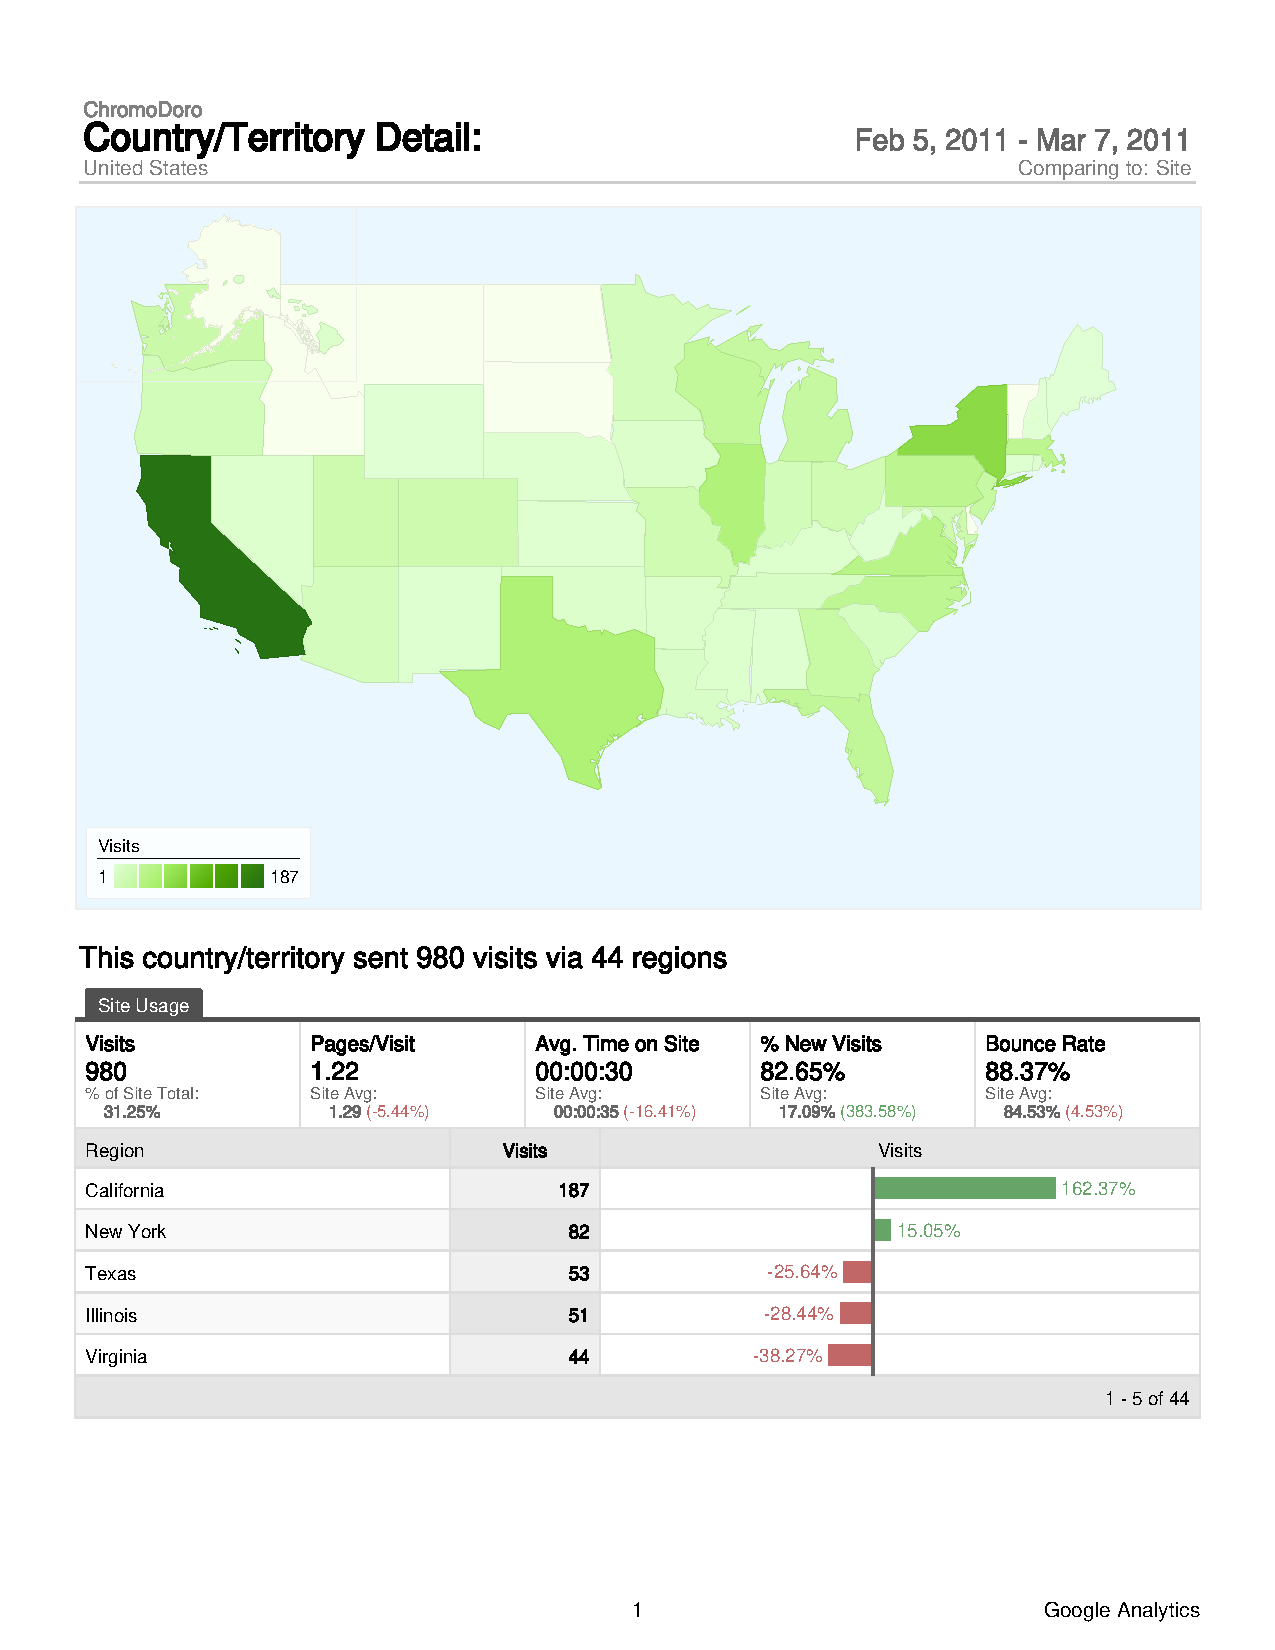
\includegraphics[width=14.25cm]{img/map-analytics.pdf}
	\caption{Google Analytics - návštěvy podle zemí}
	\label{img:analytics-map}
\end{figure}



\subsection{Sběr dat pomocí JavaScriptu}

Většina těchto informací se dá zjistit jak pomocí JavaScriptu na straně klienta, tak pomocí HTTP protokolu na straně serveru. Tato kapitola popisuje ty, které se dějí uvnitř prohlížeče a není je tedy možno měřit analýzou logovacích souborů.

Událostí v prohlížeči je třeba klik na tlačítko, psaní do textového pole, skrolování na stránce, dokonce i pohyb myší a změna velikosti prohlížeče. Jedná se o interakci uživatele se stránkou - ta probíhá v rámci prohlížeče na straně uživatele a tudíž není ji možno měřit jinak, než na straně uživatele.

K sběru dat na straně uživatele se používá JavaScript. Jedná se o skriptovací jazyk a kromě jména nemá nic společného s jazykem Java. Pomocí tohoto jazyka jsou v prohlížeči veškeré události zachyceny, zaznamenány a zpracovány.

\subsubsection{Klání myší}

Klikání myší na stránce způsobuje přechod na jinou stránku, nebo spuštění nějaké funkce. Pokud by se jednalo pouze o odkaz na jinou stránku, vystačili bychom si s analýzou logových souborů. Stránky však často obsahují aktivní prvky, které nepožadují novou stránku, ale mění pouze část stránky. 

Například foto alba umožňují větší náhled obrázku bez nutnosti přejít na novou stránku. Takovou událost je ale možno zachytit a zpracovat. Podobně ani odchozí odkazy nezpůsobují požadavek na náš server, na kterém bychom mohli provést analýzu logovacího souboru. 

Odkaz, který vede na stránku na jiném serveru, totiž nezpůsobí požadavek na náš server a je nutné ho zaznamenat už při události kliknutí v prohlížeči. Takovému odkazu, u kterého návštěvník opouští naší stránku říkáme takovému odchozí. 

Provozovatele serveru může zajímat, kam z jeho stránky návštěvníci odcházejí. Autora článku zajímá, které odkazy z jeho článku jsou nejzajímavější pro jeho čtenáře.


\subsubsection{Pohyb myši}

Pohyb myši na stránce není kritický faktor, který je třeba sledovat na všech webech jako například kliky myší. Samy o sobě nemají velkou vypovídají hodnotu, existují však nástroje, které je těchto informací dokážou využít.

Agregace pohybů myší se využívá ke konstrukci heatmap. Účel heatmap je graficky znázornit, kterým částem webové stránky se dostává nejvíce pozornosti, ty se zobrazují teplými barvami (žlutá, červená), místa kterým se nedostává pozornost jsou naopak la\-dě\-ny do studených barev (zelená, modrá).

Jiným využití znalosti o pohybu myši je mouse-tracking. Tato technika kombinuje sledování kliků a pohybů myši a tak pořizuje záznam o uživatelově činnosti na stránce. Jedná se o velmi specifickou techniku, která se používá k testování stránek ještě dřív, než se uvolní na veřejnost, nebo k optimalizaci těch částí stránky, kde dochází ke sledované konverzi. Příklad aplikace mouse-trackingu ke sledování konverze je například v proces dokončení objednávky elektronickém obchodě.



\subsubsection{Stisky kláves}

Události používání kláves se používá nejčastěji ve spojení s mouse-trackingem (viz Pohyb myši) k testování uživatelské zkušenosti, nebo k optimalizaci objednávkových formulářů v podobných situacích.

Některé webové stránky kladou velký důraz na přístupnost a umožňují uživateli se navigovat pomocí klávesových zkratek. V takovém případě by měli měřit i používání těchto zkratek a případně je upravit tak, aby byla navigace na jejich webu co nejjednodušší.




Událost skrolování stránky nastává když uživatel posouvá stránku nahoru a dolů, případně doprava nebo doleva. Podle  posuvu stránky v určitých intervalech se dá usuzovat, že uživatel stránky čte, nebo pouze prohlíží. Podle délky čtení a toho, jestli se uživatel dostal až na konec článku se dá určit, jestli článek dočetl.

V kombinací s velikostí vnitřní části okna prohlížeče se dá přesně určit, na kterou část stránky se uživatel dívá. Toho se například využívá k vykreslení heatmapy, která kolik času uživatelé věnují jednotlivým částem stránky. 


\subsubsection{Opuštění stránky}
Odchod ze stránky je událost, která je spuštěna když uživatel přechází na jinou stránku, nebo zavírá okno se stránkou. 

Tato událost se používá k vypočtení tzv "bounce rate". Jedná se o procento uživatelů, kteří na stránku přijdou a hned zase odejdou. Takové chování se dá očekávat například, když uživatel něco hledá ve vyhledávači, prohlédne si a vzápětí odchází, protože na první pohled stránka neobsahuje informace, které hledal.

Bounce rate je třeba chápat v kontextu s tím, odkud uživatel přichází. Měl by se odlišovat podle zdroje, odkud návštěvník přišel. Například návštěvníci z vyhledávače budou mít odlišný bounce rate, než návštěvníci z odkazujících článků, reklamy, nebo ti, kteří přímo napíší adresu stránky do adresního řádku.

\subsubsection{Rozlišení obrazovky}

Rozlišení obrazovky je informace která vypovídá o návštěvníkovi a zařízení, které po\-u\-ží\-vá. Starší monitory se například poznají tím, že mají poměr stran 4:3. ty novější zase 16:9 a 16:10. Stejně tak se dá usuzovat, že u pokud je rozlišení nízké, ale zároveň se jedná o širokoúhlý monitor, může se jednat o netbooky, nebo notebooky.

Nejvyšší rozlišení mají nejmodernější dvaceti sedmi a třiceti-palcové monitory. Ještě větší rozlišení jako je 3200x1200 znamená, že má uživatel více, než jeden monitor. V případě 3200x1200 se může jednat o monitory s rozlišením 1920x1200 a 1280x1024, tedy sedmnáct, až devatenácti a dvaceti čtyř palcový monitor vedle sebe.





\subsubsection{Cookies}

Díky cookies\cite{cookies} je možné rozpoznat návštěvníka stránky. Při první návštěvě se ná\-vště\-vní\-ko\-vi uloží do cookies jeho unikátní identifikátor a lze tak při příští návštěvě říct, že se jedná o stejného návštěvníka. Označování návštěvníků umožňuje zjistit například počet uni\-kát\-ních návštěvníků. Přesto, že někteří uživatelé si cookies ručně mažou, většina to nedělá a počet unikátních návštěvníků získaný pomocí cookies lze pokládat za relativně přesný.

Označování uživatelů umožňuje také sledovat počet návštěv. Pokud uživatel stráví pět minut prohlížením stránek, zavře stránku a pak se za dvě hodiny vrátí, říkáme, že šlo o dvě návštěvy.

Dlouhodobé opakování návštěv označujeme jako loajalitu návštěvníků. Stránky, které mají tuto hodnotu vysokou mají stabilní bázi návštěvníků, kteří si tam zvykli pravidelně chodit. Tato hodnota je důležitá pro informační servery, elektronické obchody, blogy, fóra a komunitní stránky.

%{\bf Doba strávená na stránce}
%\bigskip


%\bigskip


\subsubsection{Tepelné mapy}

Na obrázku \ref{img:heatmap-bing-google} je ukázka heatmapy pro stránky výsledků vyhledávačů Google a Bing. Vstupními daty pro vytvoření takových interpretací jsou v ideálním případě data získaná pomocí sledování očních pohybů návštěvníků pomocí speciální kamery. Takovéto tes\-to\-vá\-ní je možno provádět pouze v laboratoři a s potřebným vybavením.

Mimo laboratoř je možno takové obrázky vygenerovat z pohybů myší a klikání ná\-vště\-vní\-ků stránky. Cílem heatmap je odhalit, kterým částem stránky se dostává více pozornosti. Na obrázku \ref{img:heatmap-bing-google} jsou vidět heatmapy ze studie\cite{heatmap}, která porovnává, kam se uživatelé na obou stránkách nejčastěji dívají.

\begin{figure}[hp]
	\centering
	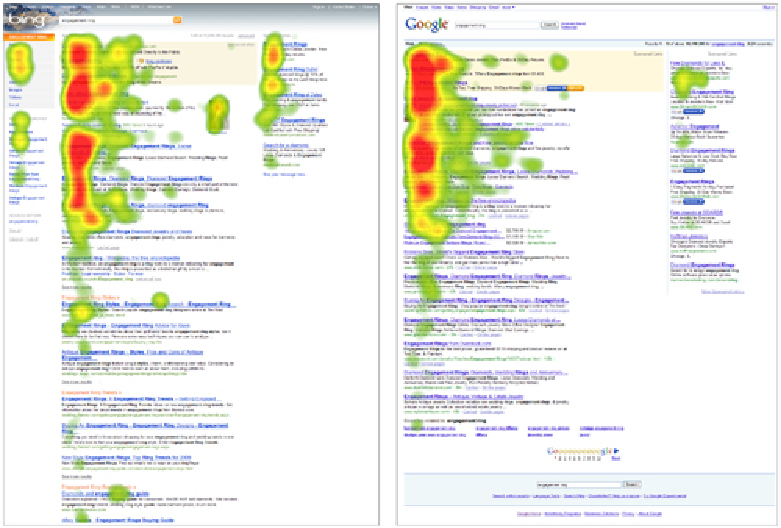
\includegraphics[width=14cm]{img/google-bing-heatmap.pdf}
	\caption{Heatmapy - vlevo Bing, vpravo Google}
	\label{img:heatmap-bing-google}
\end{figure}




%\subsubsection{Heatmapy}
%\subsubsection{Světová mapa}
%\subsubsection{Segmentace}


\subsubsection{Aplikace v praxi}

Teď, když byly nastíněny základy toho, jak webová analytika sbírá a interpretuje data je na místě se zmínit o praktickém využití těchto dat.

%Optimalizace konverze reklamních kampaní

Na počátku, kdy se měřil pouze počet zobrazení stránky, byly tyto nástroje měřítkem popularity stránek. Podle denní návštěvnosti se dalo odvodit, kolik by si měla stránka účtovat za reklamu\footnote{Dnes jsou více rozšířené systémy, které požadují platbu za počet prokliků a jejich cena se určuje formou aukce. Například AdWords, u nás Sklik.}, většinou formou bannerů. Návštěvnost stránek i dnes určuje cenu reklamy na stránce, PR článků a obecně hodnotu celé stránky.

Když potenciální zákazník klikne na reklamu a dostane se naši stránku, stojí nás to peníze. Ne každý zákazník objedná, nebo jinak vygeneruje zisk. Takže kolik zákazníků, kteří se na naši stránku dostali přes reklamu u nás vlastně nakoupí? A ještě lépe - kolik nás ve výsledku stojí nová objednávka? Na tyto otázky standardně odpovídá například Google Analytics, který je přímo napojen na AdWords\footnote{Google Adwords \url{http://adwords.google.com}}.

V okamžiku, kdy se na naši stránku dostane uživatel, vstupuje do hry měření kon\-ver\-ze\cite{conversions}. Ta měří poměr návštěv a uskutečněných cílů - například počet objednávek, nebo počet nových emailů v seznamu odběratelů novinek. Konverzní poměr se zvlášť měří u uživatelů, kteří přišli z vyhledávače, přes reklamu anebo sami napsali adresu webové stránky do prohlížeče.

Znalost jednotlivých konverzí a napojení na reklamní systém umožňuje určit cenu za konverzi a tím i efektivitu jednotlivých kampaní.



%\bigskip

%Optimalizace pro vyhledávače

Typické zdroje návštěvnosti jsou reklama, vyhledávání a dnes nově sociální média. Vyhledávače jsou kapitolou samou pro sebe. Vyhledávače používá velké denně množství lidí a je lákavé dostat svůj web do horních pozic pro vyhledávané fráze související s tématem stránky. Díky tomu, že reklama je relativně drahá je optimalizace pro vyhledávače žádanou službou, která představuje dlouhodobý nárůst návštěvnosti za jednorázovou investici.

Návštěvnost z vyhledávačů lze efektivně měřit i s zjištěním návštěvnosti pro jednotlivé klíčové slova a vyhledávací fráze. Analytické nástroje tak umožňují změřit o kolik se zvedl počet objednávek, registrací nebo čehokoli, co majitel stránky sleduje jako cíl konverze.


%Split testing

Mocným nástrojem pro optimalizaci webových stránek je split-testování, taktéž zvané A/B testování. Tato technika spočívá v tom, že se vytvoří dvě varianty stránky a něk\-te\-rým uživatelům se zobrazí jedna varianta a některým druhá. Na daných stránkách se pak měří konverze a výsledkem testu je zjištění, která stránka měla větší konverzi.

Tímto způsobem se dají optimalizovat stránky, které mají zákazníka přimět k registraci, nákupu, nebo jiné cílové akci. Tato technika umožňuje určit, jaký název produktu bude mít lepší výsledky, alternativní slogany, vzhled produktu, nebo dokonce i cenu produktu. 

V případě testování ceny produktu se některým zákazníkům zobrazí například \$19 a jiným \$49. Je docela možné, že produkt za \$49 se bude lépe prodávat, protože zákazníci od něj budou očekávat větší kvalitu. Přesto, že nezní příliš sofistikovaně, umožňuje split-testing každému experimentovat s mnoha aspekty a reálně ověřit, zda navrhované změny opravdu vedou k lepší konverzi.

%optimalizace použitelnosti patří ještě pod optimalizaci konverze



Druhá strana mince je v případě webové analytiky hlubší porozumění. Do této kategorie patří informace typu jaké prohlížeče a zařízení používají, jaký jazyk preferují, z jaké části světa jsou, odkud na stránku přicházejí, co na webu dělají a kudy stránku opouštějí. 

V závislosti na zaměřené webové stránky je tady větší nebo menší snaha poznat zákazníka. Dnešní analytické nástroje mají pouze omezené možnosti práce se zá\-ka\-zní\-kem, především z toho důvodu, že odmítají vědět o tom, že jde o konkrétního zákazníka, jako například Google Analytics, který sledování konkrétních uživatelů přímo zakazuje v podmínkách použití.

Na práci se zákazníky se specializují jiné systémy jako jsou CRM Systémy\footnote{Customer Relationship Management systémy} a jiné úzce specializované produkty, které se již webovou analytikou nezabývají. 

Právě znalost konkrétního zákazníka a práce s ním odlišuje nový analytický produkt od ostatních. V dnešní době sociálních médií, kdy telefonní operátoři mají teamy lidí, kteří se starají o zákaznickou podporu na sociálních sítích, je kritické mít přehled o svých zákaznících a to zvláště u webových aplikací, kde interakce zákazníka s aplikací je to, za co nás zákazník platí.



\subsection{Etická stránka sběru dat}

\begin{comment}
Problém etiky sběru dat.
Právní problémy.
Anonymní vs. neanonymní data.
Webaplikace vs. webová stránka.
Zákazník vs. náhodný návštěvník.
Analogie z fyzického byznysu.
\end{comment}

Záměrné zahalování identity uživatele je argumentováno zachováním soukromí u\-ži\-va\-te\-le. Například Google Analytics obsahuje ve smluvním ujednání služeb Google Analytics následující text:

\begin{quote}
7.1 Nebudete slučovat (nebo nedovolíte jakékoliv třetí osobě slučování) jakákoli data shromážděná z vaší Website (vašich stránek Website) (nebo website ta\-ko\-vé\-to třetí strany) s jakýmikoliv informacemi identifikujícími osoby, které pocházejí z jakéhokoli zdroje jsoucího částí vašeho užívání (nebo užívání takovéto třetí strany) Služby. Budete splňovat všechny zákony na ochranu dat a soukromí ve spojitosti s vašim používáním Služby a shromažďováním informací od návštěvníků na vašich stránkách website. Na své stránce na viditelném místě zpřístupníte (a budete i dodržovat) vhodnou směrnici o ochraně soukromí.
\ldots
\end{quote}

Na jedné straně je snaha ochránit uživatelovo soukromí, na druhé poskytnout co nejlepší službu a relevantní obsah. Etickou stránku věci se spíše zabývají velké firmy, které mají uloženo mnoho uživatelských dat a nezávislí profesionálové, kteří poukazují na přestupky a nedostatky.

Problém soukromí na webu je možno přirovnat k nakupování v obchodu. Pokud jsem v obchodním řetězci a nakupuji, budou mě sledovat kamery, které mě dokáží identifikovat a sbírají data o tom, kudy chodím. Z hlediska soukromí nechci, aby bez mého souhlasu o mě sbíral obchodní řetězec informace o tom, co nakupuji, jak často do obchodu chodím, nebo co mám na sobě. Toto je filosofie Google Analytics.

Když se svým nákupem přistoupím k pokladně, první na co se mě prodavačka zeptá je, zda mám jejich "kartu". Pokud ano, vezme si ji k zařízení napojeném na pokladnu a v tom okamžiku se můj zatím anonymní nákup stává mým nákupem a je svázán s mou kartou. Tímto způsobem obchodní řetězec dokáže sledovat jak často nakupuji a co nakupuji.

Aby měl zákazník důvod k pořízení karty, která umožňuje jeho sledování je motivován sbíráním bodů, nebo jinými výhodami\footnote{Například IKEA svým členům "IKEA Family" věnuje nápoje k jídlu zdarma.}. Při registraci pro kartu IKEA Family se do formuláře vyplňuje jméno, příjmení, bydliště, email a den narození. O ochraně osobních údajů říká IKEA, že jde o "vztah založený na důvěře". V následujícím výňatku z textu "Ochrany osobních údajů" společnost polopatě vysvětluje, že údaje bude poskytovat třetím stranám:

\begin{quote}
{\bf Informace, které nám sdělíte, u nás také zůstanou}\\
Kdybyste nemohli IKEA věřit, nemohli byste v ní ani nakupovat. Z toho dů\-vo\-du je pro nás ochrana vašich osobních důvodů navýsost důležitá. IKEA nesděluje vaše osobní údaje jiným firmám mimo IKEA. Informace, které nám poskytnete, využívá jen a jen IKEA. Někdy sice nastanou případy, kdy Vaše osobní údaje poskytneme některé z našich divizí v jiné zemi, ale v takových případech používáme všechny dostupné administrativní, technické i fyzické způsoby ochrany dat, abychom zabránili jejich možnému prozrazení, použití, změně či zničení. Stručně řečeno se všemi dostupnými prostředky snažíme chránit vaše osobní údaje před předvídatelným nebezpečím. V některých pří\-pa\-dech však opravdu musíme některé vaše údaje sdělit jiným společnostem, které pověříme jejich zpracováním, protože od nich chceme, aby vám poskytly určité služby. Zpracování osobních údajů probíhá v těchto případech podle našich pokynů. 
\end{quote}

Velké společnosti tedy respektují naše soukromí, ale v rámci vlastní optimalizace se nás snaží získat do svých klubů, které jim umožňují sbírat libovolná data a vyhodnocovat je.

Pro úplnost metafory o internetovém soukromí je třeba zmínit jak se k soukromí staví ti menší. Zákazník nakupuje v lahůdkářství víno a všelijaké dobroty. Lahůdkář dobře rozumí zboží a dokáže poradit a zákazník si rád nechá poradit,  protože sám není odborník a dobrou radu bere jako součást služby lahůdkářství. V této situaci nemá prodejce sepsaný dokument o ochraně osobních dat, nicméně ví, jaké zboží zákazník preferuje, jak často chodí, za kolik průměrně nakoupí a mnohdy i pro jaké příležitosti nakupuje.

To, co má lahůdkář v hlavě se ve větším měřítku nazývá Customer Relationship Management. CRM je nástroj ke shromažďování, zpracování a využití informací o zákaznících. Je to vlastně takový drobnohled, kterým se pohlíží na zákazníka jako jednotlivce. Toto kontrastuje s tím,jak data využívá firma s mnoha zákazníky, která je souhrnně analyzuje.

\bigskip

Nástroj, kterým se tato diplomová zabývá představuje řešení pro webové aplikace, které mají stovky až tisíce zákazníků, které fungují typicky na základě měsíčního před\-plat\-ného. V tomto případě je potřeba kombinovat způsoby analýzy dat velkých objemů a pohledu na konkrétní zákazníky. 

Nástroj si klade za cíl podporovat webovou aplikaci od jejích začátků až k dospělosti. Zabývá se celým životním cyklem zákazníků od jejich prvního vstupu na web, přes registraci trial verze, změnu plánu na placený a používání aplikace.

V metafoře výše se je produkt na půl cesty mezi lahůdkářem, který osobně zná vše\-chny své zákazníky a tato znalost je přidanou hodnotou služby zákazníkovi a obchodním řetězcem, který potřebuje analyzovat chování velkého množství zákazníků.









\section{Analýza webových aplikací}

Tato kapitola popisuje problém, který známé analytické nástroje zatím neřeší, a konkrétní způsob jeho řešení. Nástroje pro webovou analytiku nepracují s konkrétními zákazníky a některé dokonce zakazují jakkoli identifikovat uživatele webů.



\subsection{Webové aplikace}

S nástupem webových aplikací se mění i požadavky na analytické nástroje. Do webových aplikací vstupují uživatelská data ať už ve tradiční formě hodnot z formuláře, nebo data, které vznikají samotnou interakcí (například  malování). 

Když tedy uživatel vkládá, nebo vytváří v aplikaci data, je třeba je nějak uložit k tomu, aby mohly být později vyvolána a dalo se s nimi pracovat. Pro tento účel webové aplikace vyžadují způsob, jak unikátně identifikovat uživatele. V praxi to znamená, že se uživatel musí zaregistrovat a potvrdit svou identitu e-mailem\footnote{Stále častější alternativou se stávají identifikační autority jako Facebook, Twitter, nebo OpenId. To umožňuje, že uživatel nemusí vyplňovat email, ani heslo a je přihlášen pomocí jediného kliknutí.}.

Právě to, že je uživatel přihlášen dává nové možnosti vývoje nástrojů pro webovou analytiku. Na rozdíl od webových stránek, kde nemůžeme s jistotou určit, zda se jedná o stejného uživatele můžeme podle přihlášení s jistotou tvrdit, že se o jedná o stejného uživatele a víme kterého.

V prostředí, kde je uživatel přihlášen můžeme na data pohlížet zcela jiným způsobem. Vezměme si statistiku počtu návštěv, kterou zpracovává Google Analytics a podává ji hned na hlavní stránce statistik pro daný web. Denní počet návštěv je vypočítán tak, že pokud přijdu na stránku ráno, v poledne a večer, započítá se to jako tři návštěvy. Pro webovou stránku to dává smysl ze dvou důvodů. Zaprvé ze stejného počítače může přijít ráno v poledne a večer úplně jiný člověk a to nelze nijak rozeznat. Zadruhé webové stránky nemají uživatele, ale návštěvníky tudíž dává smysl sledovat návštěvy. 

Na druhé straně jsou aplikace, které mají uživatele a tak dává smysl sledovat po\-u\-ží\-vá\-ní. Jestli uživatel přijde třikrát denně, nebo jednou a stráví v aplikaci 3x tolik času je hezké vědět, ale není to tak podstatné. Co je podstatné je kolik uživatelů reálně dnes navštívilo aplikaci a kolik v ní strávili času.

Tento rozdíl se nezdá na první pohled až tak markantní. Je třeba si uvědomit, že se jedná o odlišný úhel pohledu a z toho vycházejí odlišné závěry. Například z Google Analytics se dá zjistit, kolik procent návštěv je z mobilních zařízení. 

Řekněme, že mobilní zařízení tvoří 3\% všech návštěv. To není jako mnoho, pra\-vdě\-po\-do\-bně neznamená, že budeme upravovat naši aplikaci speciálně pro mobilní zařízení. Na druhou stranu, pokud máme 85\% uživatelů, kteří používají free účet a 15\% platících\footnote{Freemium model, spočívá v účtech zdarma a placených, které poskytují něco navíc.}, mohou tři procenta znamenat až 20\% platících uživatelů. Pokud máme více, než jeden placený tarif, například basic (\$19), gold (\$49) a platinum (\$199). V takovém případě bude velmi důležité vědět, kolik z našich 3\% je ve kterém tarifu.

Některé věci, které jsem popsal Google Analytics umožňuje. Je pouze na uživateli, aby si svoje Analytics co nejlépe nastavil a svou aplikaci opatřil příslušným nastavením, které umožní sledovat zajímavé údaje o uživateli.

Tento univerzální přístup ovšem znamená, že co si uživatel sám neudělá, to nemá. Další omezení spočívá v tom, že Analytics zakazuje identifikovat uživatele.

Tato situace mě motivovala k vývoji nástroje, který je výhradně zaměřen na analytiku webových aplikací s důrazem na práci s uživateli. Nejedná se pouze o zpřesnění výsledků, jde o to zaměřit se na zákazníky a nikoliv na průměrná čísla.



\subsubsection{Motivace}

%Popis problému.
Webové aplikace se od webových stránek odlišují v klíčových faktorech a tak si vyžadují odlišný náhled na analýzu jejich uživatelů. 

Asi největší rozdíl spočívá v tom, jak webové aplikace a webové stránky vydělávají peníze. U aplikace platí uživatelé za její používaní, nebo za nadstandardní služby. Menší webové stránky jako například osobní blogy většinou přímo nevydělávají, ale poskytují autorovi status profesionality a odbornosti. Ty s větší návštěvností získávají peníze pomocí reklamy, affiliate programů, nebo PR článků.

V závislosti na tom, kolik používání aplikace stojí může webová aplikace potřebovat mnohem menší množství platících uživatelů, než webová stránka neplatících návštěvníků k tomu, aby vydělávala. 

Při vývoji nové aplikace potřebují tvůrci veškerou zpětnou vazbu, kterou mohou dostat. Mají jen velmi málo uživatelů a jsou s nimi v úzkém kontaktu. Takovým uživatelům se říká "early adopters" a z hlediska vývoje je spočívá jejich úloha v používání produktu a podávání zpětné vazby. 

V okamžiku, kdy se produkt dostává k většímu počtu uživatelů, není možné se všemi udržovat písemný kontakt a jen malá část je ochotna podat zpětnou vazbu. 

V tomto okamžiku nastupuje nový nástroj, který si klade za cíl poskytovat podporu pro práci se zákazníkem a životním cyklem zákazníků.


\subsection{Životní cyklus návštěvníka} % co to bude umět

Životní cyklus zákazníka je možné rozdělit chronologicky do čtyř částí. Akvizice, Uživatel, Zákazník a konec využívání aplikace. Každá fáze má své specifika a vyžaduje si trochu odlišný přístup, protože nás v ní zajímá něco jiného.

\begin{figure}[h]
	\centering
	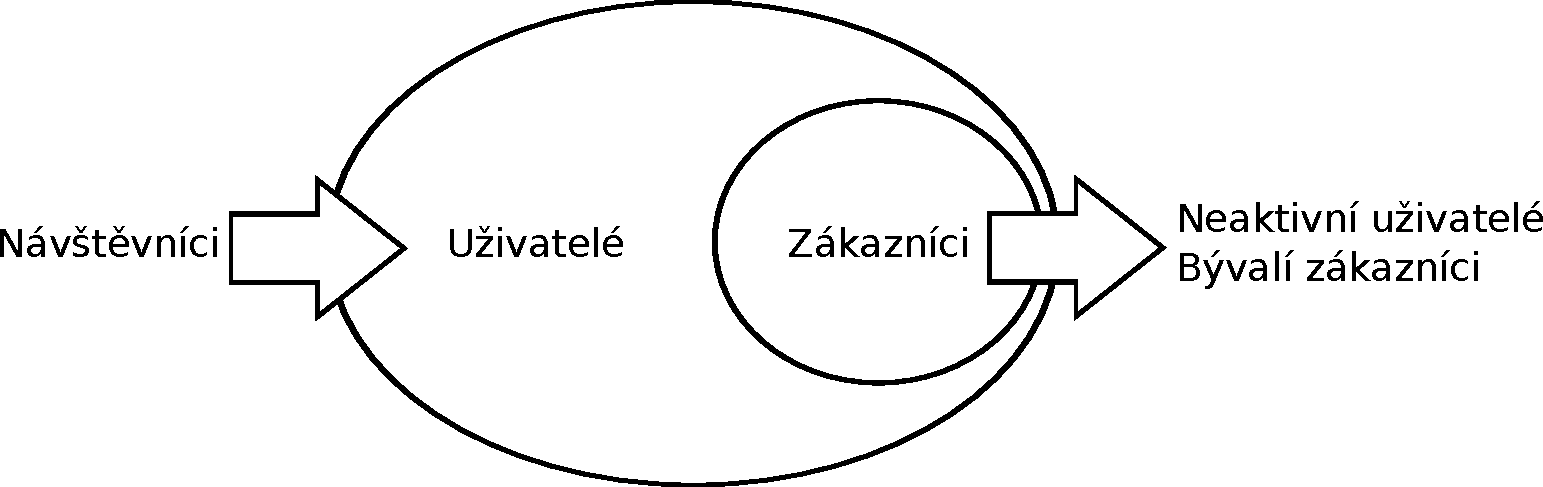
\includegraphics[width=14cm]{img/user_lifecycle_slim.pdf}
	\caption{Životní cyklus uživatelů}
	\label{lifecycle}
\end{figure}

\subsubsection{Akvizice uživatele}

Ještě než se z návštěvníka stane uživatel musí přijít na webovou stránku aplikace, kde se informuje o aplikaci. Většina nástrojů v této fázi dokáže identifikovat odkud uživatel přišel a dokáže říct, kolik návštěvníků z jakého zdroje se registruje.

Jelikož se konvenční nástroje omezují a unikátně neidentifikují uživatele, je tato funkce pouze jednorázová. To znamená dá se zjistit, že přes reklamní kampaň X přišlo sto ná\-vště\-vní\-ků a dva se zaregistrovali. Pokud se návštěvník na stránku vrátí a zaregistruje se až další den, nástroje to nezaznamenají kvůli anonymizaci dat.

Nový nástroj naopak pracuje s uživateli jako s lidmi, ne daty a tak každý uživatel nese informaci o tom, odkud poprvé přišel a kdy se zaregistroval. To znamená, že je možno zpětně zjistit ze kterých kampaní vzniklo nejvíce placených zákazníků globálně a ne jednorázově.

\subsubsection{Uživatel}

Když se návštěvník zaregistruje, stane se z něho uživatel. V tuto chvíli většina webových aplikací poskytuje třicetidenní testovací lhůtu, během které se uživatel má seznámit s produktem a pak se rozhodne, jestli ho bude platit, nebo ne. Tomuto způsobu se říká "trial verze".

Alternativou je tzv. Freemium, což znamená, že uživatel využívá základní verzi produktu a má možnost si zaplatit za prémiové funkce, nebo možnosti.

Na rozdíl od zákazníka, který za produkt platí a tudíž se dá předpokládat, že produkt vyhovuje jeho účelům a využívá ho pro svůj prospěch není u uživatele jasná motivace. 

U trial modelu mohou uživatelé používat všechny možnosti aplikace v rámci zkušební doby, používají tedy stejnou aplikaci jako ti platící. Není však jisté, že aplikaci nepřestanou používat a začnou za ní platit. Cílem je tedy nabídnout něco, co je tak dobré, že se bez toho zákazník neobejde.

Cílem freemium modelu je nabídnout něco, co uživatelé začnou používat zdarma a časem přejdou na placenou verzi. Tento model se liší hlavně v tom, že uživatelé používají nějakým způsobem omezenou verzi. Zde se opakuje to, že není jisté, že uživatelé začnou platit, podobně jako u trial verze.

Motivace platících a neplatících uživatelů se liší. Někteří uživatelé pouze hledají mo\-žnost, jak zdarma vyřešit svůj problém a nemají zájem o prémiové funkce aplikace, jiní aplikaci jenom zkoušejí a časem si najdou jinou, nebo aplikaci sice používají, ale není pro ně tak podstatná, aby za ni platili.

Neplatící uživatelé jsou ti, kteří projevili zájem o produkt, ale ještě se nestali platícími zákazníky. U freemium modelu tato skupina početně převažuje platící uživatele zhruba 10:1 a je nutno na ní pohlížet zvlášť.

\subsubsection{Zákazník}

Zákazníci jsou ti, kteří umožňují produktu žít a rozvíjet se. Tím, že platí za produkt vyjadřují tím, že jim produkt pomáhá natolik, že jej ohodnotí svými těžce vydělanými penězi. V dnešních webových aplikací, které hojně využívají freemium model se může jednat o pouhých 10\% všech uživatelů, často i méně. 

Zákazníci jsou srdcem produktu a je třeba pečovat. Několik procent zákazníků se v tom davu zbývajících neplatících uživatelů snadno ztratí a tím pádem je třeba jejich statistiku oddělit. Jelikož jde o početně menší skupinu, je také záhodno využít nástrojů, které se dívají více do hloubky a držet si tak své nejdůležitější uživatele blíž u těla. 

Můžeme identifikovat uživatele, kteří produkt používají nejčastěji, takzvané "power users". Tito znají produkt velmi dobře, možná lépe než naši zaměstnanci. V této skupině se budou pravděpodobně vyskytovat lidé, kteří se zasadili o rozšíření produktu mezi své přátele a zákazníky. Budou to lidé, kteří o produktu často mluví a dělají mu dobré (nebo taky špatné) jméno.

Power users mohou pomoci s testováním nových funkcí, poskytnout dobrou referenci produktu, mohou se také stát evangelisty pro daný produkt, kteří ho propagují s oficiální podporou. O tuto skupinu je třeba se dobře starat, být s ní v kontaktu a naslouchat jim. 

Na druhou stanu, mezi power uživateli se mohou vyskytovat i takoví, kteří produkt jednoduše přerostli a ten se už nehodí pro jejich účely. Toto je možné detekovat například monitorování funkcí, které používají a porovnání s ostatními zákazníky.

Další podskupinou, o kterou je třeba se zajímat jsou noví zákazníci. Ti buď produkt už znají z doby, kdy používali neplacenou verzi, anebo jsou noví. Když zákazník začne platit, neznamená to, že bude produkt stále používat. Novým zákazníkům je možno nabídnout pomoc, poslat jim dopis s video tutoriálem k používání produktu, nebo je například po určité době používání oslovit, poděkovat jim a zeptat se, jak se jim produkt používá.

Je také třeba sledovat, zda uživatelé, kteří začali platit produkt používají a v případě že ne, oslovit je a zjistit proč. Je možné, že produkt nepochopili, nebo třeba nevyhovuje jejich účelům. Někteří dokonce mohli zapomenout, že produkt začali používat (pokud se to ještě nestalo jejich zvykem). Takto je možné získat nedocenitelnou zpětnou vazbu, podle které je možno upravit prezentaci produktu, doplnit sekci "Často kladené otázky", nebo upravit produkt tak, aby sám naučil uživatele, jak ho mají používat. 

Takto lze dlouhodobě snížit počet zákazníků, kteří produkt opouští. Nejen, že si u\-dr\-ží\-me víc zákazníků, ale získáme přidanou hodnotu pro náš produkt, podle toho jak ho upravíme, aby se dobře a jednoduše používal.




\subsubsection{Konec používání aplikace}

Určitá část uživatelů přestane používat náš produkt. Možná náš produkt nevyhovuje jejich vzrůstajícím požadavkům, přecházejí na konkurenční produkt, nebo již nepotřebují takový produkt vůbec používat. Ať už je důvod jakýkoli, strávili s naším produktem nějaký čas a pokud se jednalo o platící zákazníky, tak u nás zanechali i peníze a umožnili tak našemu produktu růst.

Je zde určitý trend, kdy se podnikatelé a firmy snaží hrát na lidskou notu. Pokud to myslíme vážně, toto je vhodný čas, kdy jim můžeme odeslat poděkování za celou tu dobu strávenou s námi. Pěkný děkovný email podepsaný ředitelem společnosti zanechá v zákazníkovi pocit, že u této společnosti nebyl jen dalším číslem ale opravdu člověkem a pokud to souhlasí s tím, jak se k němu poskytovatel aplikace choval v průběhu používání, je velká šance, že produkt dále doporučí, vrátí se, nebo zmíní, jak se k zákazníkům u této společnosti chovají.

Děkovný dopis je také dobrým místem, kde je můžeme dát zákazníkovi prostor, aby se vyjádřil k tomu, proč odhází a ukázat, že nám na něm záleží.

\bigskip

Tímto končí životní cyklus zákazníka a popis motivace k vývoji nového nástroje. Dále bude popsáno jaké funkce nástroj obsahuje a jakou roli hrají v celku.










\subsection{Vlastnosti nástroje}


Tato podkapitola se věnuje tomu, co nový nástroj dělá, proč a jak. Zaměřuje se v první řadě na uživatele a podporuje čtyři fáze jejich životního cyklu: návštěvník, uživatel, zá\-kaz\-ník a bývalý zákazník, nebo uživatel.

Tedy přidanou hodnotou produktu je to, že kopíruje životní cyklus uživatele a je úzce zaměřený ná práci s uživateli. Na rozdíl od ostatních analytických nástrojů, které jsou neposkytují žádné základní přizpůsobení pro daný typ aplikace a už vůbec nepracují s konkrétními uživatel.

Každá fáze životního cyklu je v nástroji reprezentována jako pohled, který zobrazuje jednotlivý segment takovým způsobem, který umožňuje získat ty informace, které nás u dané skupiny zajímají. Toto rozdělení umožňuje vnímat výsledky měření v kontextu a poskytuje základní segmentaci uživatelů.



\subsubsection{Návštěvníci}

Tento pohled zobrazuje pouze segment návštěvníků. Návštěvníkem myslíme toho, kdo se ještě nezaregistroval do aplikace. V rámci životního cyklu zákazníků je návštěvník chápán jako potenciální uživatel, nebo zákazník. Návštěvník se stane uživatelem v o\-ka\-mži\-ku, kdy se zaregistruje a zvolí "free" plán u freemium produktu, nebo placený plán s časově omezenou verzí.

Návštěvníky můžeme rozdělit na nové a vracející se. Počet nových a vracejících se zákazníků umožňuje určit, zda se o naší stránce dovídá dostatečné množství nových návštěvníků a kolik z nich se po první návštěvě vrací. 

Z hlediska konverze návštěvníků na uživatele nás bude zajímat, kolik času průměrně trvá, než se návštěvník stane zákazníkem, případně kolik návštěv, nebo zobrazení stránek. Zajímavé je taky porovnat jaké stránky navštívili návštěvníci, kteří se následn registrovali a porovnat je s těmi, kteří se nezaregistrovali.

Když přijde návštěvník na stránku naší aplikace, bude nás v první řadě zajímat, odkud přišel a v okamžiku, kdy se zaregistruje se přiřadí k jeho profilu. Z dlouhodobého hlediska to umožňuje určit, který zdroj návštěvnosti přinesl největší počet uživatelů. 

U reklamních kampaní tento dlouhodobý náhled umožňuje spočítat celkové ROI\footnote{Return of invest - návratnost investice}, které je určeno jako poměr zisku, na investovanou jednotku, viz rovnice \ref{eq:roi}.

\begin{equation}\label{eq:roi}
ROI = \frac{(Zisk - Investice)}{Investice}
\end{equation}

Uvažujme reklamní kampaň, kde jeden proklik stojí korunu. Ze sto návštěvníků se pět zaregistruje, takže cena nového uživatele je dvacet korun. Jaká je v tomto případě návratnost investice? To zatím nevíme, protože není jasné, kolik z těch pěti uživatelů se stane zákazníky a zároveň netušíme, jak dlouho u nás zůstanou.

Abychom mohli spočítat ROI potřebujeme, abychom věděli dvě věci. Za prvé je třeba znát, kolik procent uživatelů se průměrně stane zákazníky. Za druhé musíme vědět, jak dlouho naši zákazníci produkt používají a popularity jednotlivých plánů. Pak můžeme předvídat návratnost investice následovně:


\begin{equation}\label{eq:roi2}
Investice = CenaZaProklik / Konverze = 5 / (0.05 * 0.1) = 100
\end{equation}

V našem teoretickém případě stojí proklik pět korun, pět procent návštěvníků se stane uživateli a dvacet procent z nich se stane zákazníky. Z toho vyplývá, že cena za platícího zákazníka je 500 korun.


\begin{equation}\label{eq:roi3}
Zisk = PocetMesicu * MesicniZisk = 15 * 300 = 4500
\end{equation}

Tímto způsobem můžeme odhadnout návratnosti investice.

\begin{equation}\label{eq:roi4}
ROI = \frac{(Zisk - Investice)}{Investice} = \frac{(4500 - 1000)}{1000} = 3.5
\end{equation}

Číslo tři a půl znamená, že z každé investované koruny jsme udělali tři a půl koruny. Takovéto výpočty se dnes dělají pomocí průměrných odhadů, pokud si ovšem někdo nedá tu práci a sám si tento výpočet udělá ručně za použití reálných dat.

Pokud nástroj spolupracuje s webovou aplikací, lze vypočítat ROI jednotlivých kampaní pomocí reálných hodnot. Jeho působnost se ale neomezuje pouze na reklamní kampaně, ale na libovolnou formu u které je možno identifikovat zdroj návštěvnosti jako PR články, výměnné odkazy, vyhledávání a sociální sítě.

\bigskip

Ve fázi návštěvníků jde tedy primárně o to, odkud přicházejí, co na stránce dělají a jak z nich udělat uživatele. O tomto poskytuje pohled návštěvníků přehled pomocí relevantních grafů a tabulek.




\subsubsection{Uživatelé}

Tento pohled poskytuje přehled o uživatelích aplikace. Za uživatele považujeme člověka, který se zaregistroval a používá produkt zdarma (Freemium), nebo v časově omezenou (Trial) verzi.

Noví uživatelé produkt zkoušejí, zjišťují, co produkt dokáže a učí se s ním zacházet. Tito lidé ještě nemají s  produktem většinou zkušenost, je však možné, že již používali podobný produkt. V této fázi je velmi snadné o ně přijít. Nic neplatí, takže nemají co ztratit a pokud si ještě nezvykli pravidelně aplikaci používat, je pro ně velmi snadné s tím přestat. 

Proto je dobré sledovat, zda noví uživatelé produkt používají a případně je během periody, kdy produkt požívají zdarma se jich zdvořile zeptat, jak se jim s ním pracuje a připomenout, kde najdou pomoc, pokud by se jim s něčím nedařilo.

Účelem této fáze je, aby si zákazník na produkt trochu zvykl a mohl se pak rozhodnout, zda si produkt předplatí, nebo ne. Toto je krásný příklad "win-win", kdy benefituje jak zákazník, tak poskytovatel.

Tento pohled se zaměřuje na segment uživatelů a přehled o tom, kolik nových u\-ži\-va\-te\-lů se zaregistrovalo, kolik jich přešlo na placený plán v porovnání s dlouhodobým průměrem. Po stránce používání produktu pak poskytuje přehled o tom, jaké funkce produktu u\-ži\-va\-te\-lé používají a porovnání s ostatními skupinami.

Pohled poskytuje také pokročilou segmentaci uživatelů, podle toho jak dlouho a jak často aplikaci používají na nové zákazníky, pokročilé a ty, kteří aplikaci přestali používat.


\subsubsection{Zákazníci}

Zákazníci jsou ti uživatelé, kteří již platí. Tento pohled se příliš neliší od pohledu uživatelé, také obsahuje segmentaci zákazníků na nové, stálé, "power" a neaktivní uživatele.

V tomto pohledu se navíc zobrazuje u jednotlivých uživatelských skupin měsíční výdělek a je možno je segmentovat podle toho, jaký mají předplacený plán. 

Pokud zákazník poskytuje data o tom, jaké plány zákazníci využívají otevírají se možnosti reálného výpočtu ROI u jednotlivých kampaní a hlubší analýzu zákaznické báze.

Otevírají se také možnosti, které se blíží systémům pro management vztahů se zá\-kaz\-ní\-kem a vyhodnocování ziskovosti zákazníků v poměru s náklady na zákaznickou podporu a tak dále. Tyto možnosti jsou potenciálním rozšířením nástroje do budoucna, jsou však nad rámec této práce.


\subsubsection{Bývalí zákazníci}

Tento pohled končí životní cyklus zákazníka. Karta s bývalými zákazníky poskytuje souhrnnou statistiku toho, kolik zákazníku odešlo, jak dlouho strávili používáním aplikace a odkud se o aplikaci poprvé dověděli.

Údaje tohoto pohledu poskytují dlouhodobou retrospektivu.




\section{Technické řešení}

Tato kapitola popisuje technické řešení aplikace a použité technologie. 



\subsection{Sběr dat}

Nástroj sbírá data dvojího charakteru. V první řadě jde o interakci s webovou aplikací, podle které se určuje jak často uživatel aplikaci používá a jaké funkce používá. V druhé řadě jde o informace o uživateli, což umožňuje v analytickém nástroji s uživateli dále pracovat.

Zaznamenávání uživatelské interakce s aplikací probíhá ve webovém prohlížeči, který zaznamenává, jak uživatel aplikaci používá pomocí sledování událostí. Pomocí skriptu na straně klienta jsou sledovány jsou kliky myší v jednotlivých částech aplikace. U těch se zaznamenává jejich pozice ve struktuře stránky, která jednoznačně určuje jestli uživatel kliknul na odkaz, tlačítko, nebo jiný element. Tyto data jsou následně odeslána do analytické aplikace, kde jsou zaznamenána do databáze.

\begin{figure}[h]
	\centering
	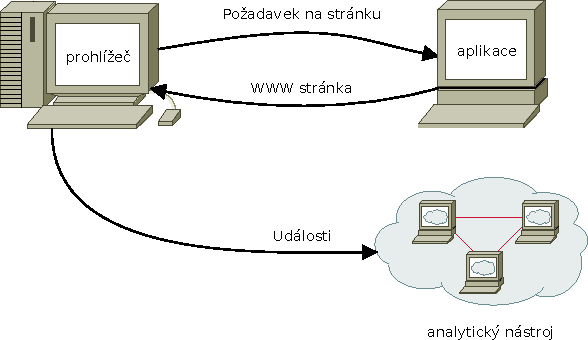
\includegraphics[width=14cm]{img/measuring.pdf}
	\caption{Schéma sběru dat}
	\label{img:measuring}
\end{figure}

Spolu se zaznamenáváním uživatelovy interakce s aplikací jsou sbírána data, která umožňují segmentoval uživatele podle toho, jestli jsou přihlášení, registrovaní, nebo jestli se jedná o zákazníky. Identifikace uživatelů spolu s jejich interakcí umožňuje segmentovat jednotlivé uživatele podle toho, jak často s aplikací pracují a dále vyhodnocovat nejpoužívanější funkce aplikace podle jednotlivých skupin uživatelů.

Na obrázku \ref{img:measuring} je obecně zachyceno, jak probíhá komunikace mezi uživatelovým pro\-hlí\-že\-čem, webovou aplikací a analytickou aplikací.


Měření je založeno na měřícím skriptu, který je vložen do webové aplikace a měření interakce, a zároveň poskytuje informace o uživateli. Jelikož se jedná o data uživatele, jsou zašifrována pomocí tajného klíče kryptograficky bezpečným způsobem.

Jelikož je nutné na straně webového serveru bezpečně zašifrovat informace o uživateli, je nutné pro každý jazyk na serveru poskytnout měřící kód v takovém jazyce, který se na serveru používá. Například kód pro jazyk PHP vypadá následovně:

\begin{lstlisting}[label=src:neco,language=PHP, caption=Měřící kód na straně serveru (PHP)]
$measuring = new UseDrivenMeasuring("chYmaXapl6Gl1VfRbGWfNA==");
echo $measuring->code(array(
    "id" => 0,
    "name" => "John Smith",
    "email" => "john.smith@example.org"
  ));
\end{lstlisting}

Zbytek kódu na serveru bezpečně zašifruje dané informace a jeho výstupem je měřící skript, který se vloží do HTML stránky. Tento měřící skript obsahuje číslo, které identifikuje webovou aplikaci, zašifrované informace o uživateli a skript, který vloží kód, který zaznamenává uživatelovu interakci se stránkou a odesílá data.

Zašifrované informace o uživateli jsou nečitelné třetí stranou a není je možno podvrhnout třetí stranou. To také umožňuje použít tuto informaci k ověření identity uživatele.

\begin{lstlisting}[label=src:html,caption=Měřící skript,language=HTML]
<script> 
  var __ud = __ud || [];  
  __ud.push(["id", 5001]);
  __ud.push(["s", "7lINfXL3mM7GEgO2HSVf9RjJS5eb9mDuVv7ba3QksTXD2BsMvadDPeU-CoIzid5PDqJI6gCOi0EjmEGtI6XSDbu9at9vY8fw6rwssCDJVA2dfuZYF7kDwzpjzivNO OfAXQls78FzwcjDhc-gxwHohMAa0l9mb7MMlV5JcDDnx7A"]);
  (function() {
    var script = document.createElement("script");
    script.type = "text/javascript"; script.async = true;
    script.src = "http://www.use-driven.com/measure.js";
    var s = document.getElementsByTagName("script")[0]; 
    s.parentNode.insertBefore(script, s);
  })();
</script> 
\end{lstlisting}


Po načtení stránky do prohlížeče je pomocí měřícího kódu dodatečně nahrán skript, který umožňuje samotné měření. Tento postup kopíruje běžně používaný způsob měření. Výhodou tohoto způsobu je především možnost měnit měřící skript bez nutnosti zásahů zeč strany provozovatele webového serveru.

Během toho, kdy uživatel pracuje s webovou aplikací měřící skript zaznamenává interakci a ukládá ji do cookie. Jedná se primárně o to, které prvky aplikace uživatel používá. Zaznamenávají se jednotlivé kliky na prvky na stránce, spolu s jejich pozicí v hierarchii dokumentu.

V okamžiku, kdy je v cookie několik událostí, posílá měřící skript nasbíraná data analytické aplikaci spolu se zašifrovanými informacemi o uživateli. Agregace událostí umožňuje snížit počet interakcí s analytickým serverem několikanásobně a tak snížit náklady na provoz.

Po přijetí dat na serveru je ověřena jejich autenticita pomocí zašifrovaného kódu. Pokud kód souhlasí jsou data jsou zaznamenána a později analyzována.







\subsection{Zpracování dat}

Nasbíraná data je nutno nějak zpracovat a interpretovat. Způsob zpracování musí být takový, aby umožňoval data zpracovat jednou a dále pak využívat pouze výsledky tohoto zpracování. To znamená, že je třeba pracovat s nasbíranými daty jako s proudem a postupně zpracovávat nová data jak přicházejí. Výstup zpracování bude pak uložen do databáze a nebude nutno data znova procházet.

Pro zvolenou metodu musí být také dostatečně jednoduché definovat nová pravidla, která data vyhodnocují. Z těchto důvodu byla vytvořena obecná forma zpracování dat jednoduchým průchodem, který umožňuje zpracovávat data po částech. Každé pravidlo, které generuje statistiku pracuje s proudem nasbíraných dat tak že navštěvuje každou událost a systém se dále nestará co s daty dělá.

\begin{figure}[h]
	\centering
	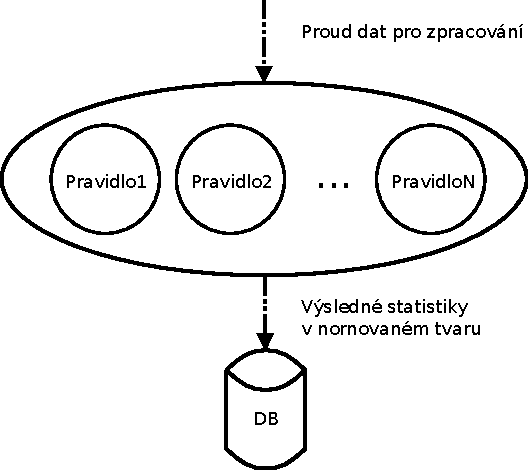
\includegraphics[width=8cm]{img/zpracovani_2.pdf}
	\caption{Schéma proudového zpracování dat}
	\label{img:measuring}
\end{figure}

Výstupem pravidel jsou dvou, nebo třírozměrné data, které jsou jednotně uložena do databáze. To umožňuje po nějaké stanovené době se zcela zbavit původních dat a ponechat si pouze z nich vyrobené statistiky, které zabírají méně místa v databázi. Po přidání nových pravidel je také možno získat jejich výsledky zpracováním dat, která již byla zpracována.

Obrázek \ref{img:metric_counter} znázorňuje třídní diagram pro třídy, které produkují veškeré statistiky. Využívám v tomto případě návrhový vzor návštěvník\cite{visitor} spolu s metodami, které zajišťují přetrvání stavu počítání tak, aby ho bylo ukončit a pokračovat později.


\begin{figure}[h]
	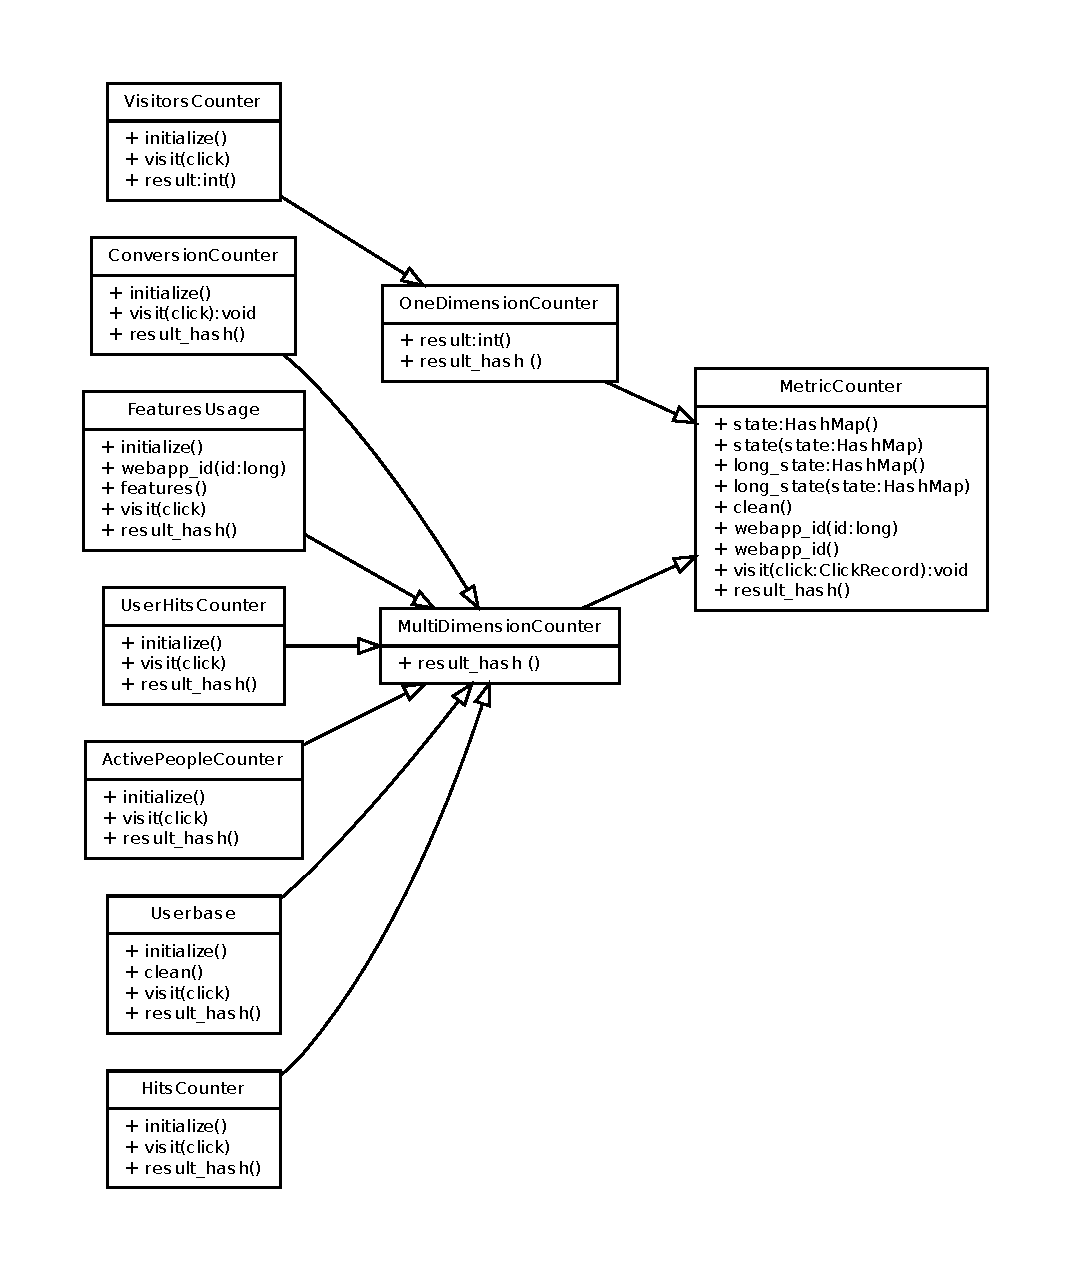
\includegraphics[width=15.25cm]{img/code/MetricCounter.pdf}
	\caption{Třídní diagram metrik}
	\label{img:metric_counter}
\end{figure}






\begin{comment}

\subsection{Struktura aplikace}

\begin{figure}[h]
	\centering
	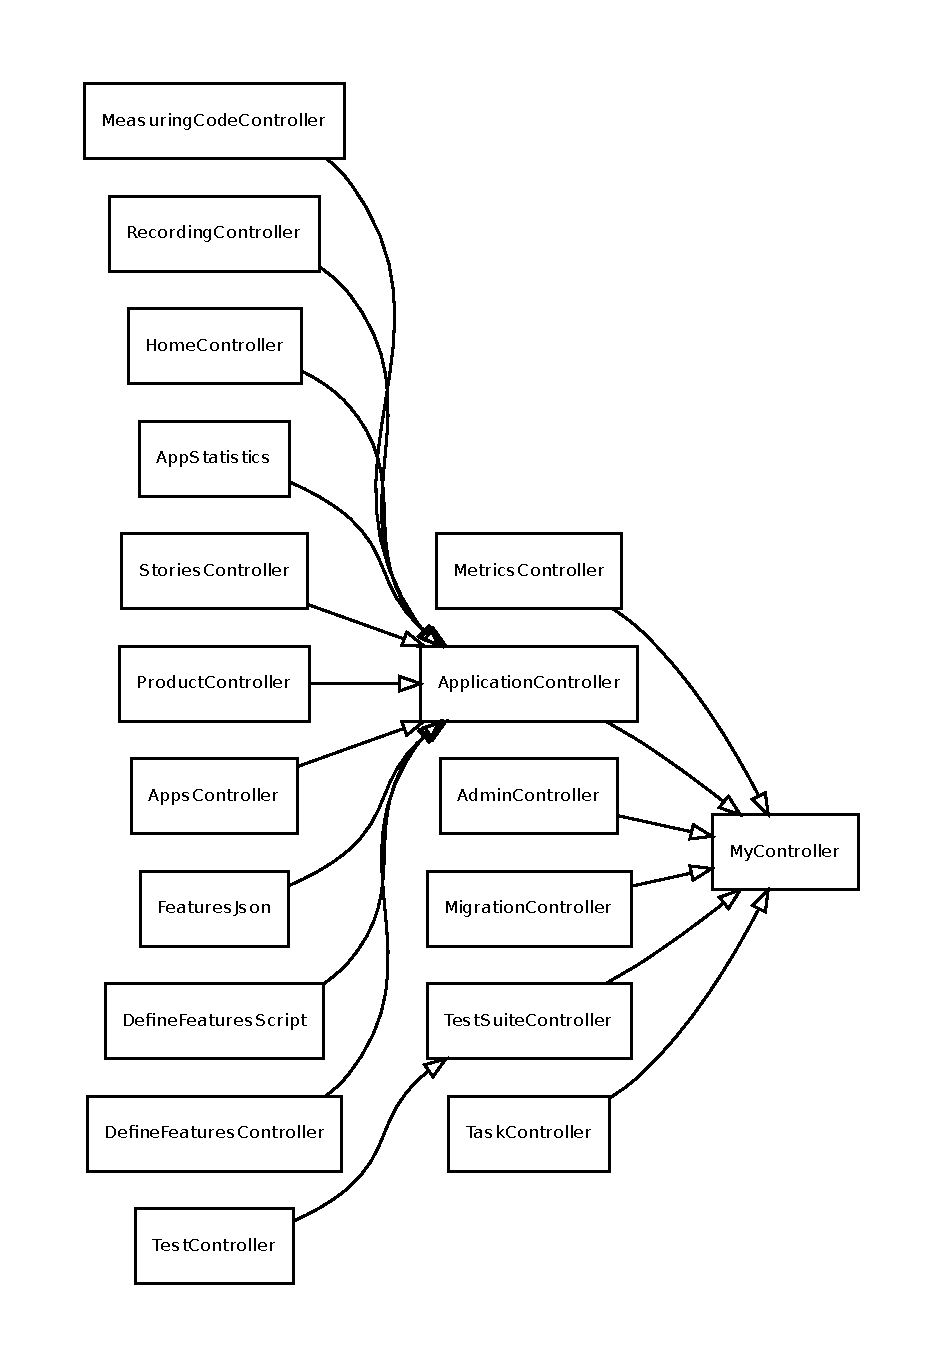
\includegraphics[width=14cm]{img/code/MyController.pdf}
	\caption{Diagram dědičnosti controllerů}
	\label{graph:my_controller}
\end{figure}

\e{comment}












\begin{comment}
	\begin{figure}[h]
		\centering
		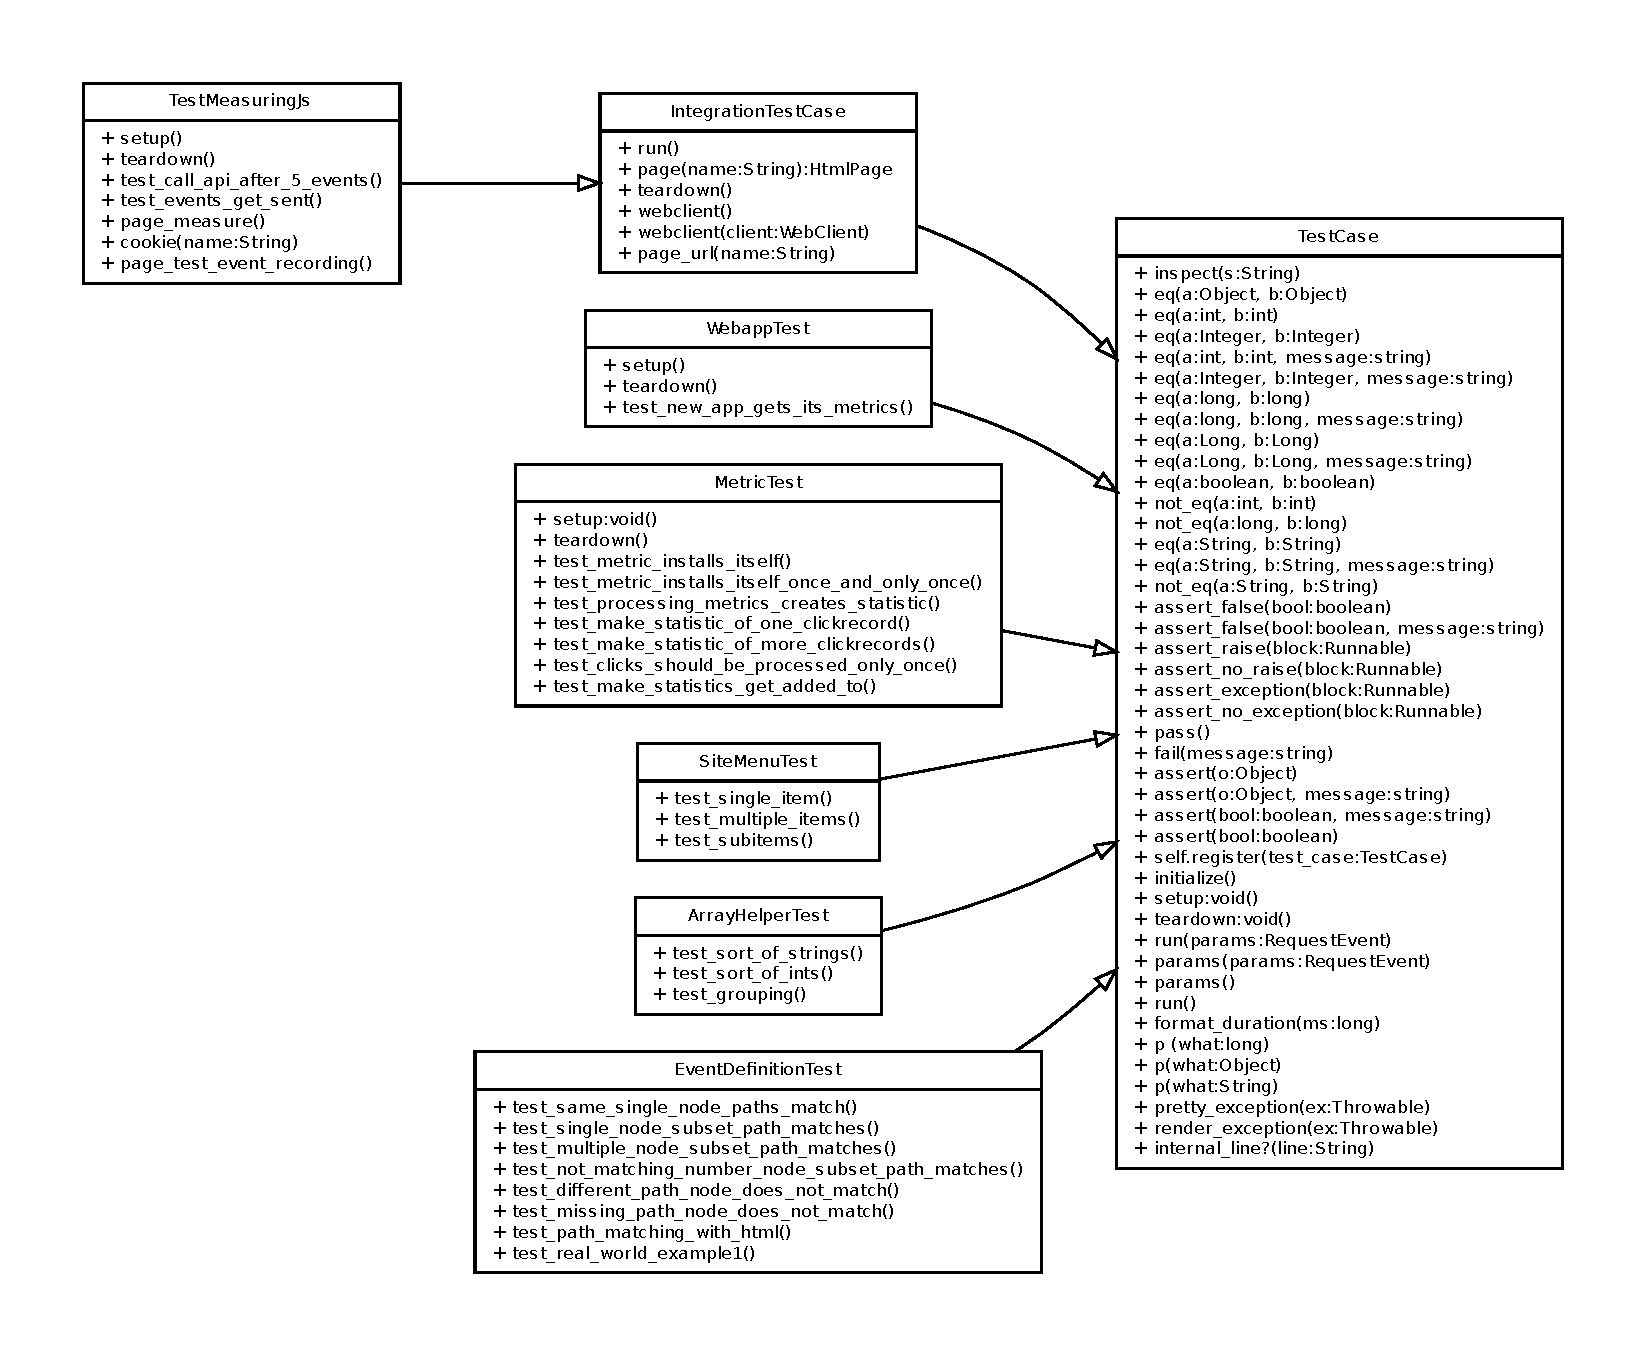
\includegraphics[width=15cm]{img/code/TestCase.pdf}
		\caption{Testy aplikace}
		\label{graph:test_case}
	\end{figure}
\end{comment}





\clearpage

\subsection{Použité technologie}

Jako platformu pro implementaci nástroje byl zvolen Google AppEngine. Jedná se službu, která je provozována společností Google od roku 2008 a vznikla jako platforma pro vývoj webových aplikací. Jedná se o službu typu "Software as a Service", která poskytuje šká\-lo\-va\-tel\-né výpočetní zdroje a zároveň softwarovou platformu pro vývoj aplikací.

Díky tomu, že AppEngine poskytuje vlastní platformu pro vývoj software, umožňuje maximálně využít potenciál cloud computingu. Díky tomu, že sleduje vytížení aplikace, je schopný v okamžiku zvýšení zátěže nastartovat nové instance aplikace, které pak postupně vypíná, když zátěž klesne. Většina operací v aplikaci jsou ve skutečnosti voláním API a ty zase může zpracovávat jiný stroj, s menší zátěží. 


\begin{comment}
\bigskip
\begin{tabular}{p{6cm} p{4cm} p{2cm}}
Zdroj							& Jednotka 				& Cena\\
\hline
Příchozí data					& gigabajt				& \$0.12\\
Odchozí data					& gigabajt				& \$0.10\\
Čas procesoru					& CPU hodina			& \$0.10\\
Uložená data					& gigabajt měsíčně		& \$0.15\\
Vysoce replikovaná databáze		& gigabajt měsíčně		& \$0.45\\
Odeslání emailu					& adresát				& \$0.0001 \\
Vždy zapnuto					& N/A (denně)			& \$0.30 \\
\end{tabular}
\bigskip
\end{comment}

Na Google AppEngine je možno programovat v Pythonu, nebo v Javě. Prostřednictvím Javy je pak možno na AppEngine provozovat aplikace napsané v libovolném jazyce, který se do Javy kompiluje, nebo je v Javě napsán. Mezi ty populární patří například JRuby (Ruby pro Javu), Groovy (dynamická java), Scala, JavaScript, Closure. 

Já jsem si zvolil jazyk Mirah, který je poměrně nový a kompiluje se do Java bytekódu. Oproti ostatním jazykům má velkou výhodu v tom, že nevyžaduje žádnou runtime library. Filosofie Mirah je použít syntaxi inspirovanou jazykem Ruby pro psaní Javy. Mirah má "pod kapotou" čistou Javu a nic víc a jde o jazyk s identickým výkonem jako má Java. Na výpisech \ref{src:fib_java} a \ref{src:fib_mirah} je možno porovnat jak se oba jazyky liší.



\begin{lstlisting}[label=src:fib_java,caption=Hello World servlet v Javě]
public class Controller extends HttpServlet {
	protected void doGet(HttpServletRequest request, HttpServletResponse response) throws ServletException, IOException {
		String name = "stranger";
		if (request.getParameter("name")) {
			String name = request.getParameter("name");
		}
		String welcomeMessage = "Welcome "+name+"!";
		response.setContentType("text/html");
 
		PrintWriter out = response.getWriter();
		out.println("<html>");
		out.println("<head>");
		out.println("<title>A very simple servlet example</title>");
		out.println("</head>");
		out.println("<body>");
		out.println("<h1>"+welcomeMessage+"</h1>");
		out.println("<form>Input your name and hit OK:");
		out.println("<input type=\"text\" name=\"\"/>");
		out.println("<input type=\"submit\" value=\"OK\"/></form>");
		out.println("</body>");
		out.println("</html>");
		out.close();
	}
} 
\end{lstlisting}



\begin{lstlisting}[label=src:fib_mirah,caption=Hello World servlet v Mirah,language=Ruby]
class Controller < HttpServlet
	def doGet(request, response):void
		name = request.getParameter(:name) || "stranger"
		welcome_message = "Welcome #{name}!"
		response.setContentType("text/html")
 
		out = response.getWriter
		out.println <<-HTML
<html>
	<head>
		<title>A very simple servlet example</title>
	</head>
	<body>
		<h1>#{welcome_message}</h1>
		<form>Input your name and hit OK:
			<input type="text" name=""/>
			<input type="submit" value="OK"/>
		</form>
	</body>
</html>
		HTML
		out.close
	end
end
\end{lstlisting}

Použitá databáze je Google Datastore, distribuovaný úložný systém, který si Google vyvinul pro vlastní potřeby. Datastore používá technologii BigTable\cite{bigtable}, která je původně navržena pro potřeby Googlu. Podmínkou bylo zvládat obrovské objemy dat, které jsou distribuovaně uloženy na tisících serverů s replikovanými daty. Na technologii BigTable běží na například Google Finance, nebo Google Earth.

Z hlediska rozdílů návrhu oproti klasické relační databázi neobsahuje datastore tabulky a sloupce, nýbrž entity a atributy. Když například v MySQL přejmenuji sloupec, změní se název sloupce u všech záznamů. Datastore pojem sloupec nezná a pokud chci nutně přejmenovat atribut u entity, je nutné projít každou entitu a změnit ji.

Dalším významným rozdílem je absence cizích klíčů a dotazů, které skládají tabulky. Dotazy do databáze jsou také značně zjednodušeny. Například pokud chci vyselektovat uživatele, kteří se zaregistrovali v určitém období mohu v dotazu omezit výsledky pouze z jedné strany a seřadit je podle omezujícího atributu. Během posílání záznamů z databáze pak přestanu požadovat další záznamy, když detekuji překročení maximální hodnotu omezujícího atributu.

Datastore tedy tlačí na programátora, aby zjednodušil logiku aplikace a omezil slo\-ži\-tost databázového schéma. Veškeré dotazování a třídění záznamů se pak děje pomocí před\-de\-fi\-no\-va\-ných indexů. Dokud uživatel nedefinuje index, nemůže podle atributu dotazovat, nebo seřazovat záznamy.

Na obrázku \ref{img:datastore_indexes} je výpis všech indexů mojí aplikace. AppEngine je sám obhospodařuje a v případě vytvoření nového indexu chvíli trvá, než je dostupný. Informace o zpracování indexu je vidět na obrázku ve žlutém rámečku.

\begin{figure}[h]
	\centering
	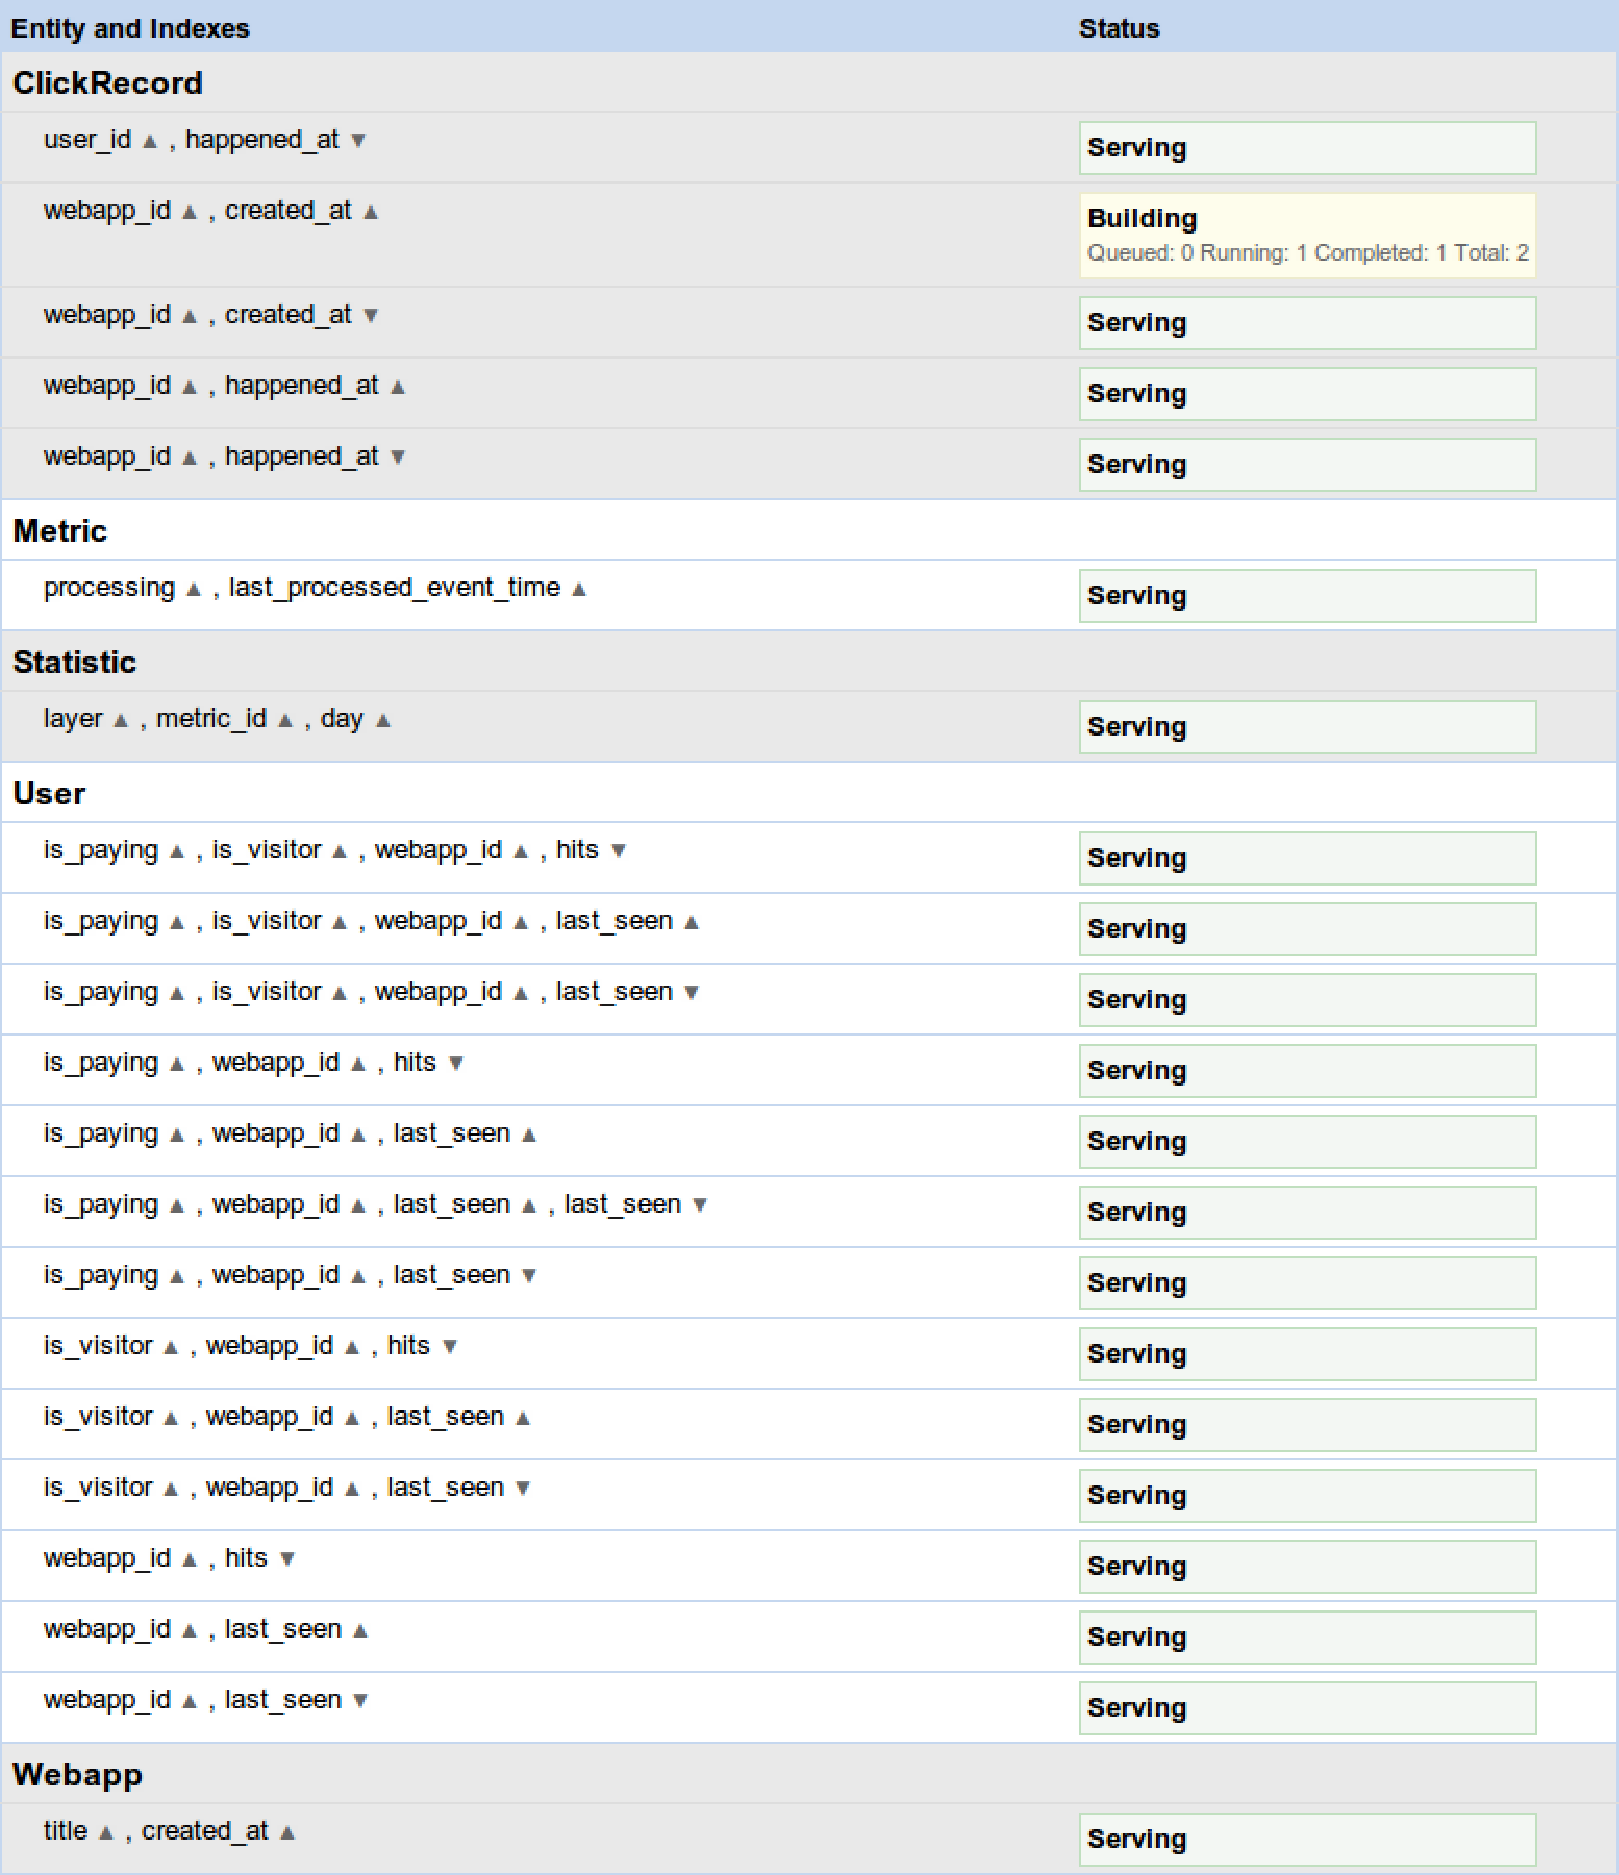
\includegraphics[width=15cm]{img/datastore_indexes.pdf}
	\caption{Indexy definované v Google Datastore}
	\label{img:datastore_indexes}
\end{figure}


\begin{comment}
Mimo databáze umožňuje AppEngine sdílení správy aplikace, uživatelské role, přehled vytížení, logování, časové spouštění úloh, profiler, statistiky používání databáze a díky tomu, že jazyk Mirah běží se kompiluje do Javy je možno také využít velké množství knihoven pro speciální účely.

\begin{figure}[h]
	\centering
	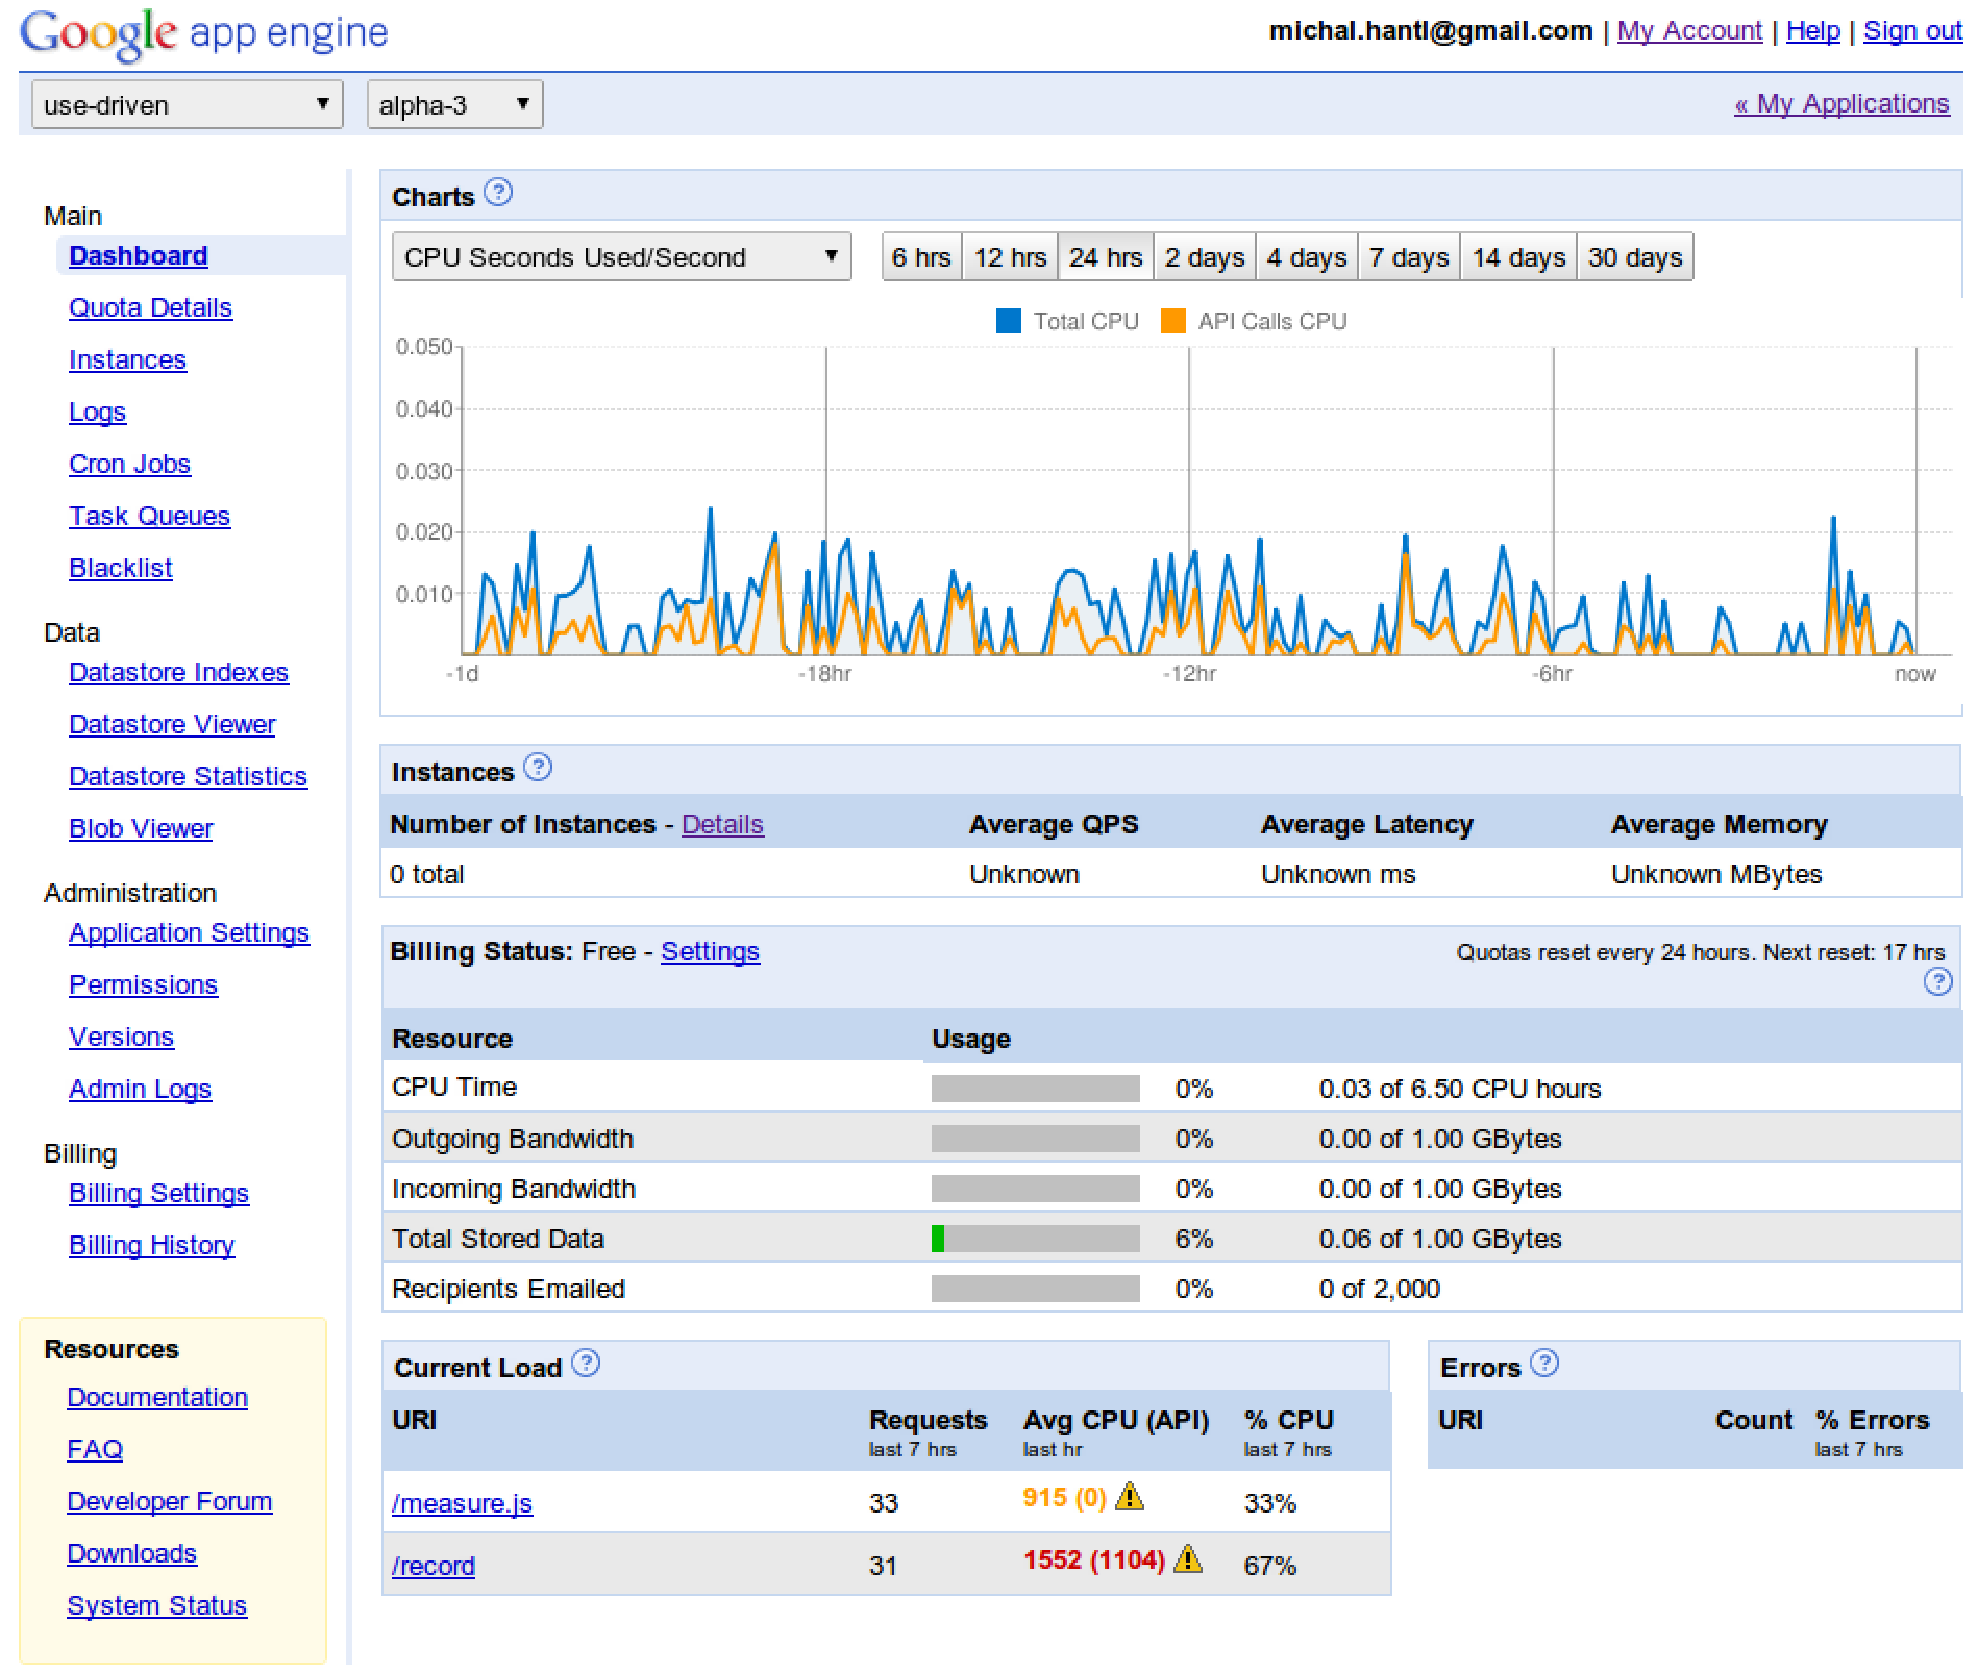
\includegraphics[width=15cm]{img/appspot.pdf}
	\caption{Administrační rozhraní platformy Google Appengine}
	\label{img:appengine_admin}
\end{figure}



\end{comment}

\clearpage
\subsection{Uživatelské rozhraní}

Při tvorbě uživatelského rozhraní jsem vycházel z toho, na co jsou zvyklí uživatelé Google Analytics. Navigace kopíruje segmentaci statistik na návštěvníky, uživatele a zákazníky. Celkově je rozhraní navrženo tak, aby bylo jednoduché a neubíralo místo na monitoru grafům a tabulkám.

Pro tvorbu grafů byly použity grafy Google Chart Tools\cite{chart_tools}, které jsou poskytovány zdarma. Vybral jsem je hlavně kvůli dobré dokumentace a množství příkladů na webu.


\begin{comment}
\begin{figure}[h]
	\centering
	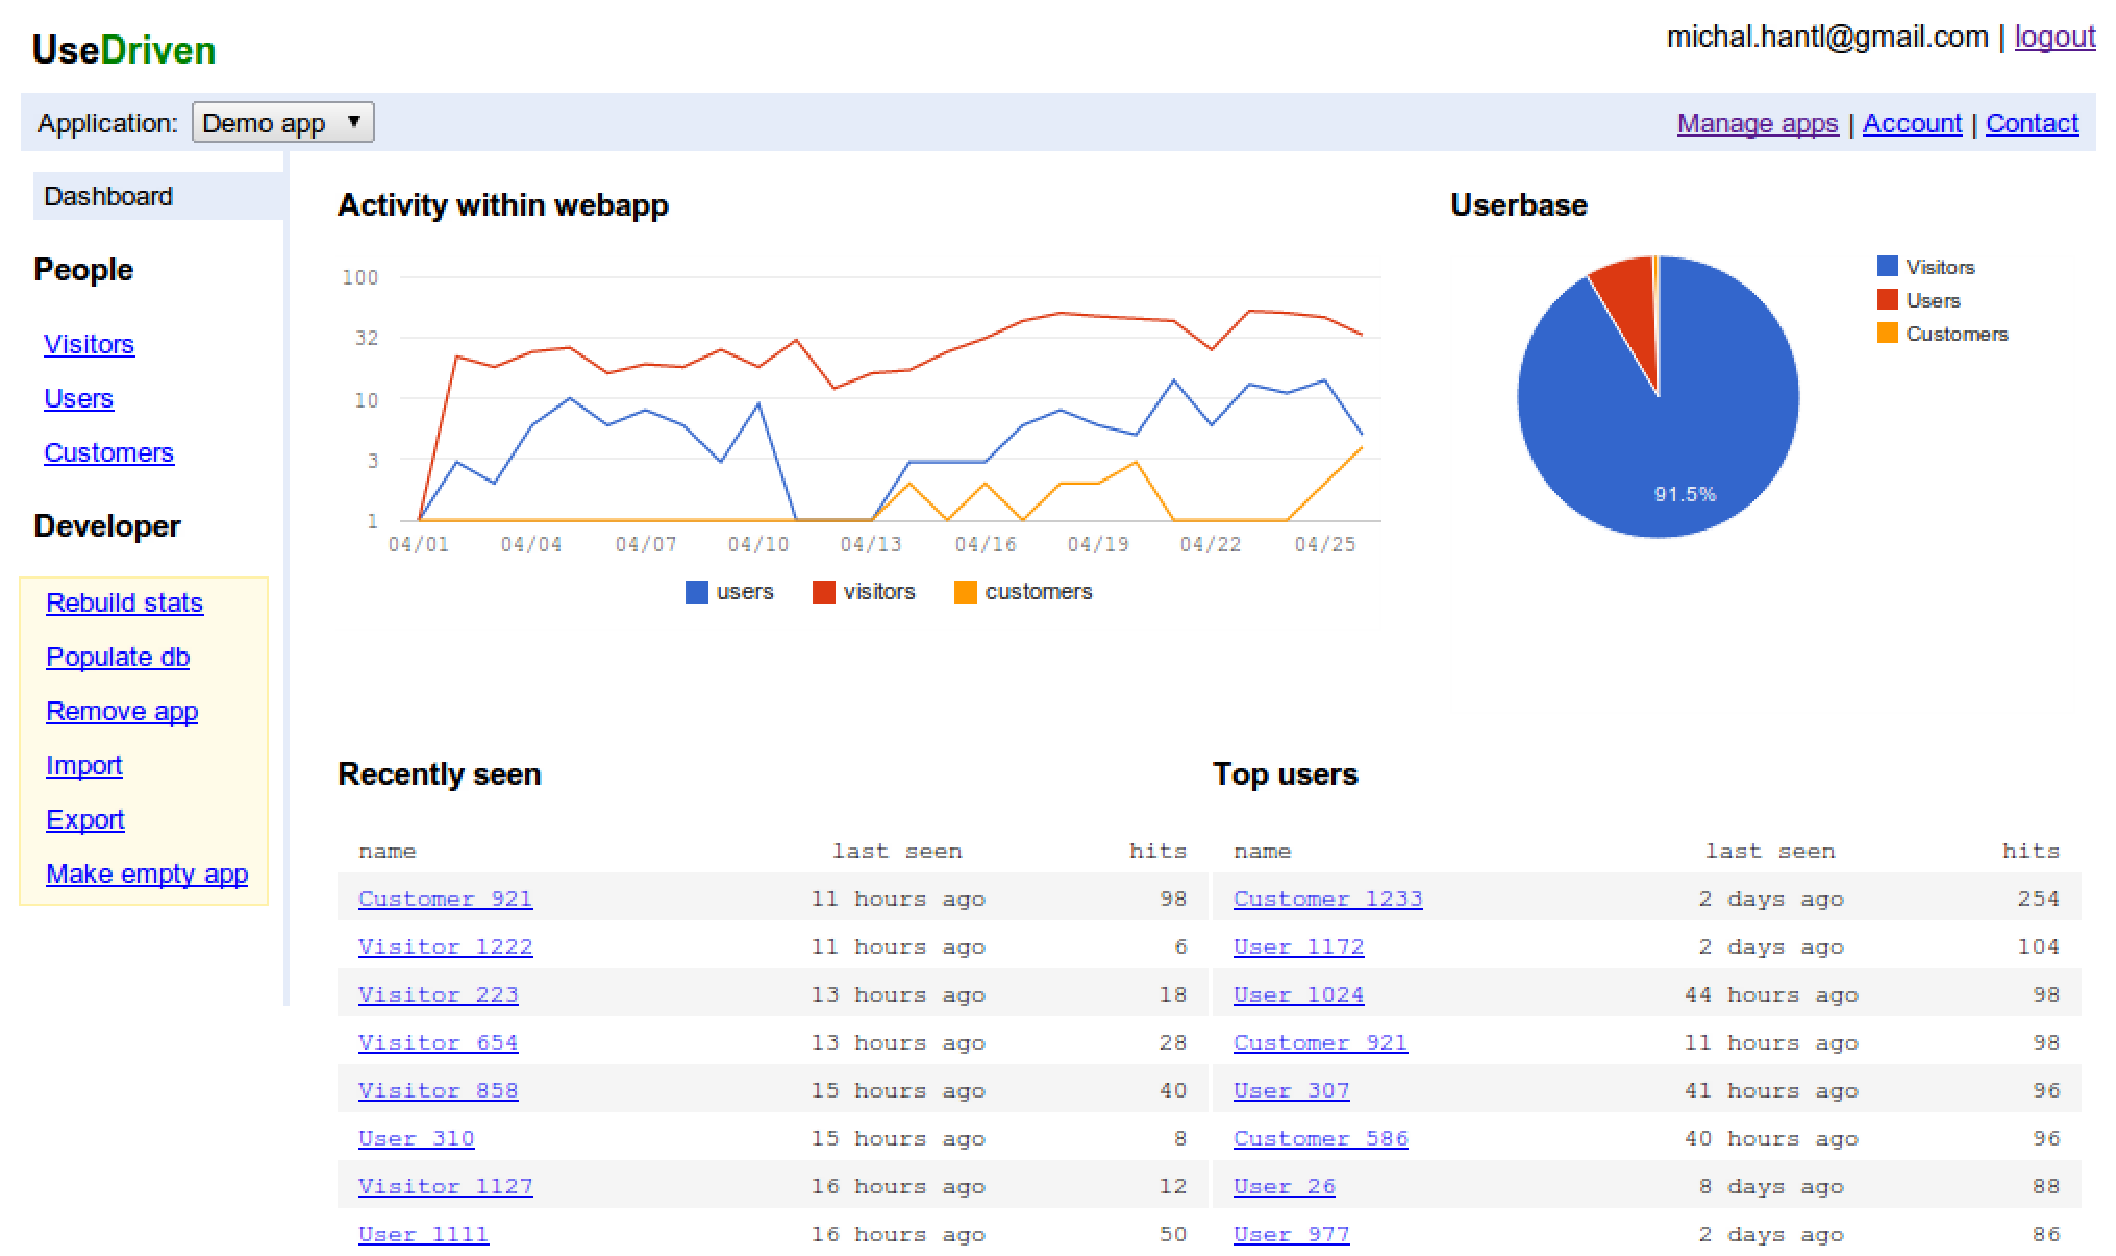
\includegraphics[width=15cm]{img/ud_dashboard_2.pdf}
	\caption{Hlavní panel aplikace}
	\label{img:ud_dashboard}
\end{figure}
\end{comment}


\begin{figure}[h]
	\centering
	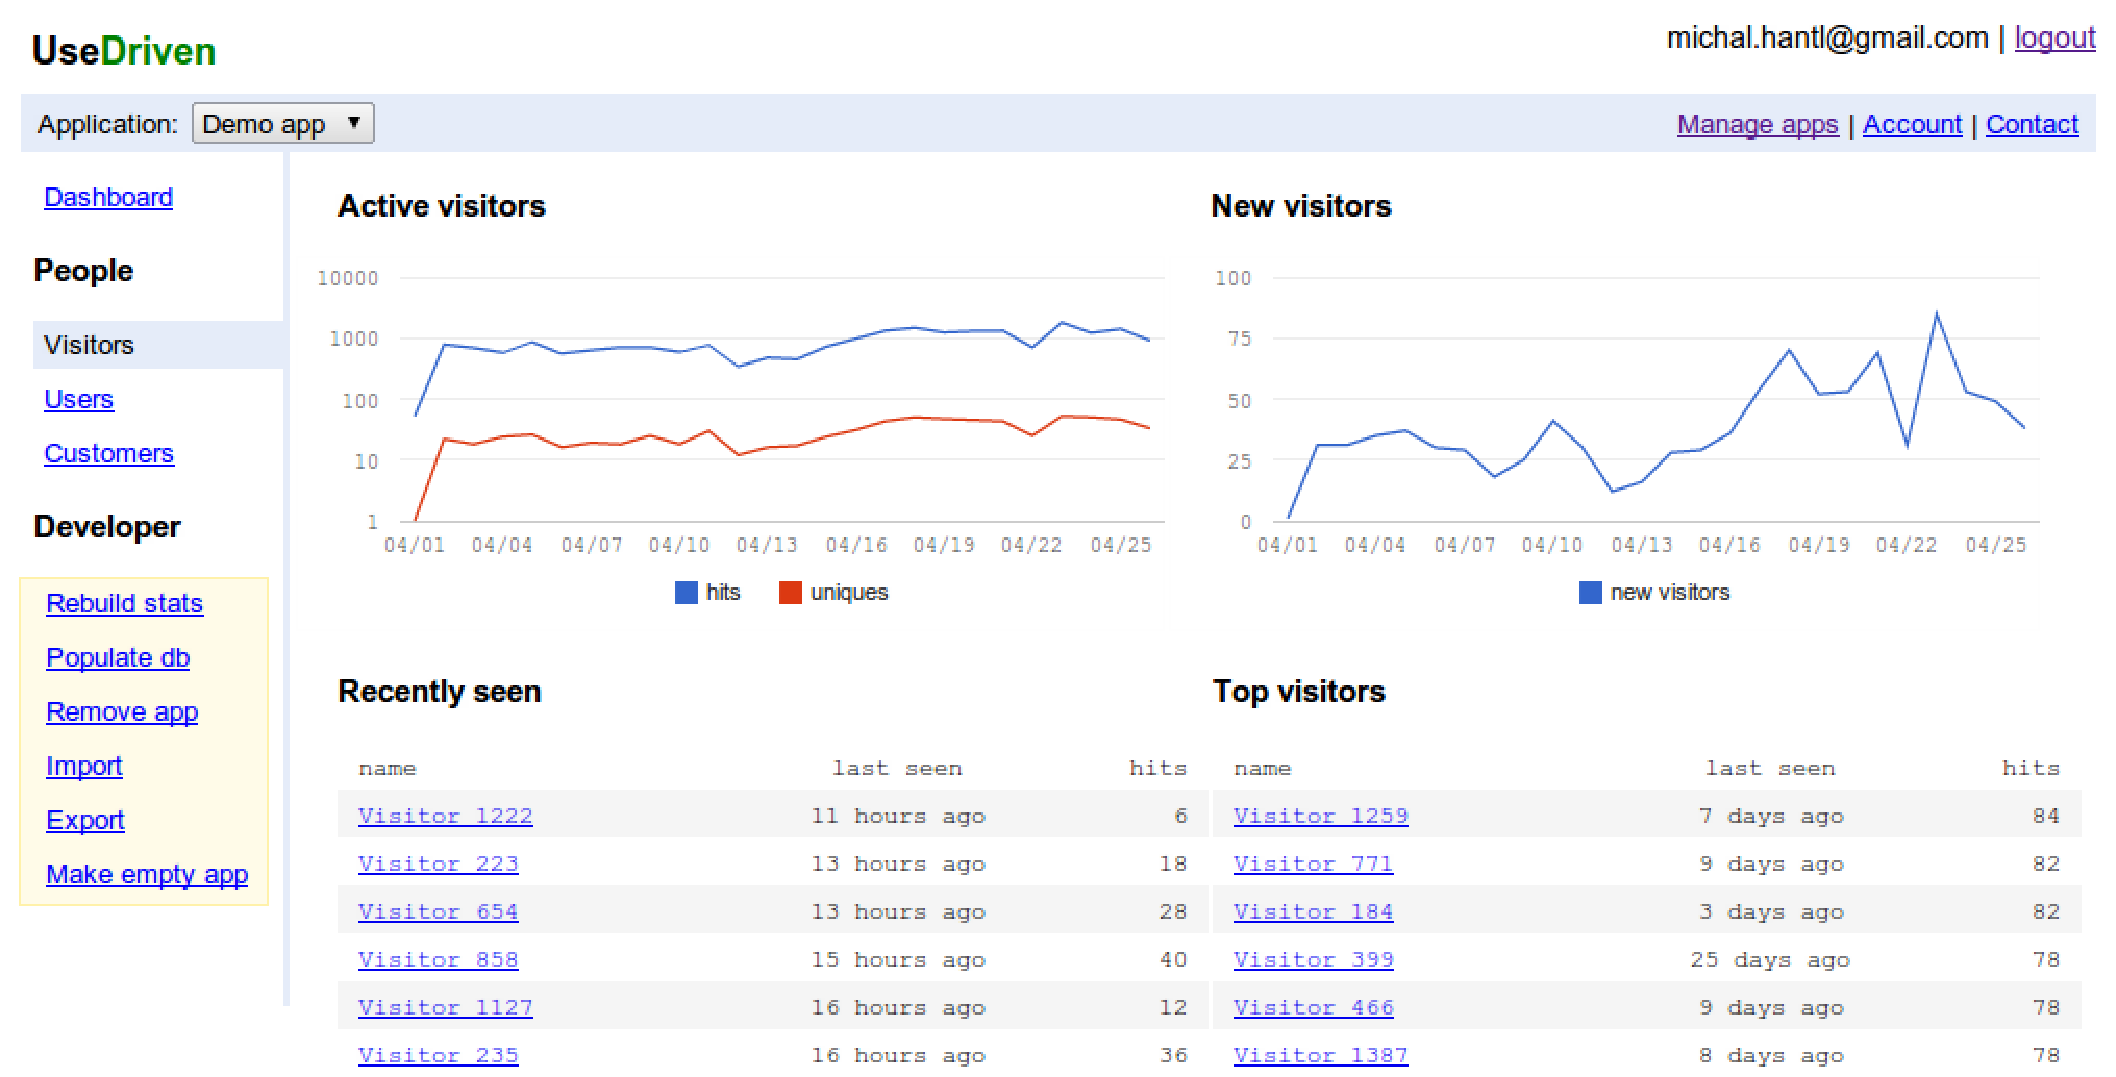
\includegraphics[width=15cm]{img/ud_visitors_2.pdf}
	\caption{Přehled návštěvníků}
	\label{img:ud_dashboard}
\end{figure}














\section{Případová studie}

Na závěr této práce jsem se rozhodl vyvinutou aplikaci otestovat v reálném provozu. Cílem bylo zajistit, že je vyvinutá aplikace schopná nasazení do běžných webových aplikací, získat zpětnou vazbu a zkušenosti z provozu. 

Vyvinutou aplikaci jsem nasadil u amerického startupu Chum.ly\footnote{http://chum.ly}. Pro tento startup jsem měl možnost měsíc pracovat. Poprosil jsem zakladatele o krátký popis toho, jak Chum.ly začalo, kde je a kam směřuje.

\begin{quotation}
CHUM.LY provides a single point of presence for reading and posting to your other social networks, as well as a local community blogging experience, where you can create or join public and private groups with shared interests.

Chum.ly began in August, 2009, with the idea of creating a central blog platform that could connect to other social networks and exceed the 140 character limit of SMS and Twitter. We used version 8 of Laconica open source code as a starting point.

Chum.ly has continued to refine the user interface and capabilities, driven by core user feedback and aided by core user community involvement. This involvement has enabled us to introduce features that are ahead of the curve, and later adopted by 'the big guys', such as inlined media and language translation. 

The 'revenue model' and 'target market' have changed numerous times, and we believe we have finally found a sustainable non-advertising-based model. However, the most rewarding part of the experience, thus far, has been the friendships forged within the Chum.ly core user community.
\end{quotation}

Uvádím také volný překlad do češtiny.


\begin{quote}
CHUM.LY poskytuje pro čtení a odesílání do jiných sociálních sítí v jednom místě, stejně jako komunitní blogy, kde si můžete vytvořit, nebo připojit se k veřejné, či soukromé skupině se společnými zájmy.

Chum.ly vzniklo v srpnu 2009, s nápadem vytvořit centrální platformu, která by mohla propojit blog s dalšími sociálními sítěmi a překročit omezení 140 znaků v SMS zprávě, nebo na Twitteru. Jako výchozí bod jsme použili jsme open source softwaru Laconica verze osm.

S pomocí zpětné vazby od a podporováno komunitou uživatelů pokračovalo Chum.ly ve vylepšování uživatelského rozhraní a funkcí. Tato podpora nám umožnila zavést prvky, které jsou na špici, které byly později adoptovány velkými sociálními sítěmi. Jedná se především o vkládání médií do zpráv a překládání.

Byznys model a cílový trh se mnohokrát změnily a věříme, že jsme konečně našli udržitelný ne-na-reklamě-založený model. Nicméně, nejvíce odměňující část zkušeností doteď, bylo přátelství v rámci komunity Chum.ly uživatelů.
\end{quote}



V Chum.ly jsem se zabýval uživatelským rozhraním a mou hlavní prioritou bylo zjednodušit ovládaní aplikace a nejlépe poukázat na vše nadbytečné, co by mohlo být eliminováno. Tento úkol mě inspiroval k tomu abych se začal zabývat tím, jaké funkce aplikace jsou používány, kým a jak často. Z této myšlenky vznikl původní nápad vytvořit aplikaci, která monitoruje používání jiné webové aplikace na základě znalosti uživatelů.


\subsection{Spuštění na ostrém serveru}

Aplikace je vyvinuta pro spuštění na platformě Google AppEngine. Jedná ze o takzvaný "PAAS", Platform as a Service. Životní cyklus vývoje aplikace vypadá tak, že je aplikace vyvíjena na lokálním stroji a je pak vypuštěna na server. Samotné spuštění na serveru bylo bezproblémové. Prostředí serveru však nekopíruje domácí a proto bylo třeba upravit několik částí aplikace.

Největším rozdílem je množství paměti na serveru, které je omezeno tak, že ne\-u\-mo\-žňu\-je pracovat s padesáti tisíci záznamy najednou v paměti. Toto bylo nutno upravit, stejně jako omezení na maximální velikost odpovědi serveru na jeden megabajt. Obě tyto omezení jsem překročil, když jsem importovat a exportoval data mezi lokálním počítačem a serverem. Pro export a import jsem tedy vyvinul nástroj, který tato omezení obchází a pracuje s libovolným množstvím dat po částech.

Omezení paměti a nároky na dlouhodobé zpracování dat po částech dalo vzniknout abstrakci nad sekvenčním zpracováním měřených dat. Umožňuje zpracovávat nové data po libovolně velkých částech, kdykoli přestat a zase začít ve stejném stavu a místě, kde bylo zpracovávání ukončeno. Zavedení abstrakce také podstatně zjednodušilo vytváření nových metrik a logiku aplikace.

Nové data tedy aplikace zpracovává po částech pomocí časovaného úkolu, který předává zpracování dat jednotlivým metrikám a v univerzálním formátu je zaznamenává do databáze.

Z praktických důvodů také došlo k optimalizaci měřícího skriptu tak, aby odesílal data v dávkách několika událostí najednou. Snížily se tak řádově nároky na procesorový čas na serveru (za který se platí) a tak i cena jeho provozu\footnote{AppEngine poskytuje 6.5 hodin procesorového času denně zdarma, ten jsem ani jednou nepřekročil.}.

Měřící skript byl upraven aby fungoval ve všech běžných prohlížečích, jeho kód byl komprimován\footnote{Komprimace JavaScriptu proběhla pomocí Google Closure Compiler \url{http://code.google.com/closure/compiler/docs/gettingstarted_ui.html}} pro minimální velikost pro co nejrychlejší přenos na stranu klienta. Výhodou platformy AppEngine je v tomto případě i to, že statická data na serveru jsou poskutována pomocí CDN\cite{cdn}, která zajišťuje co nejlepší dostupnost souborů a tímpádem i měřícího skriptu.

Optimalizace měřícího skriptu je završena kešováním, které ponechává skript v pro\-hlí\-že\-či dva dny a nemusí ho po tuto dobu znova nahrávat. Tyto technky jsou běžně využívány měřícími nástroji, které používají měřící skript. Oproti zavedeným nástrojům jako je Google AppEngine je měřící skript velmi malý, lehce přes tisíc znaků. Zatímco sofistikovanjší AppEngine používá skript o délce přes dvacet tisíc znaků.

V průběhu 55 dní, kdy aplikace běžela a sbírala data jsem ji dále vyvíjel a vznikaly tak nové verze. Při nahrávání nových verzí na server se může snadno stát, že se něco pokazí, a aplikace přestane měřit, nebo fungovat. Díky použití platformy AppEngine bych v  takovém okamžiku mohl přepnout aplikaci na předchozí a předejít tak ztrátě dat. Za dobu vývoje jsem takovýto problém naštěstí neměl.

Během běhu aplikace nedošlo k žádným větším problémům. Pouze k krobnostem a jednalo se spíše o poznatky z ostrého provozu, které měly za výsledek zdokonaletí vnitřností aplikace. Získal jsem tím i lepší znalost platofrmy AppEngine, se kterou jsem začal experimentovat zhruba před necelým rokem.


\subsection{Získaná data}

Zaznamenávaná data se skládají výhradně z událostí kliknutí na stránce. Každé kli\-knu\-tí je reprezentováno časem, ve kterém nastalo a umístěním v HTML dokumentu. Po ka\-ždých pěti až patnácti kliknutích jsou měřícím skriptem data odeslána na server a ten je vyhodnocuje.

Za sledované období padesáti pěti dní bylo zaznamenáno šedesát tisíc kliknutí. Zá\-zna\-my těchto kliků a výsledky jejich zpracování v databázi na AppEngine zabraly 24 megabajtů. Na platformě AppEngine se zvlášť platí\cite{billing} za místo, čas procesoru a další služby. Spotřeba těchto služeb je uvedena v tabulce \ref{tab:consumption}.

\bigskip


\begin{table}
	\centering
	
\begin{tabular}{p{3.25cm} p{2.5cm} p{2cm} p{2.5cm} p{2cm}}
zdroj					& jednotka & cena		& čerpání denně	& měsíčně \\
\hline
Příchozí data			& gigabajt				& \$0.12	& 0.01			& \$0.036 	\\
Odchozí data			& gigabajt				& \$0.10	& 0.01			& \$0.03	\\
Čas procesoru			& CPU hod.				& \$0.10	& 0.08 			& \$0.24	\\
Uložená data			& gigabajt				& \$0.15	& 0.03			& \$0.135	\\
\hline
						& 		 				& 			& 				& \$0.441 \\
\end{tabular}
	
	\caption{Spotřeba zdrojů při měření aplikace Chum.ly na Google AppEngine}	
	\label{tab:consumption}
\end{table}


Dlouhodobě bylo v měřené aplikaci denně třicet uživatelů a každý den vzniklo prů\-měr\-ně kolem tisíce kliků. Tato návštěvnost podle tabulky \ref{tab:consumption} generuje měsíčně náklady za 45 centů. Pokud by se jednalo o zákazníka s desetinásobným počtem aktivních uživatelů, bude se jednat o náklady zhruba ve výši čtyř dolarů měsíčně. Z toho vyplývá rámcově jakým způsobem by zákazník za tuto aplikaci měl platit - podle počtu aktivních uživatelů.

\begin{figure}[h]
	\centering
	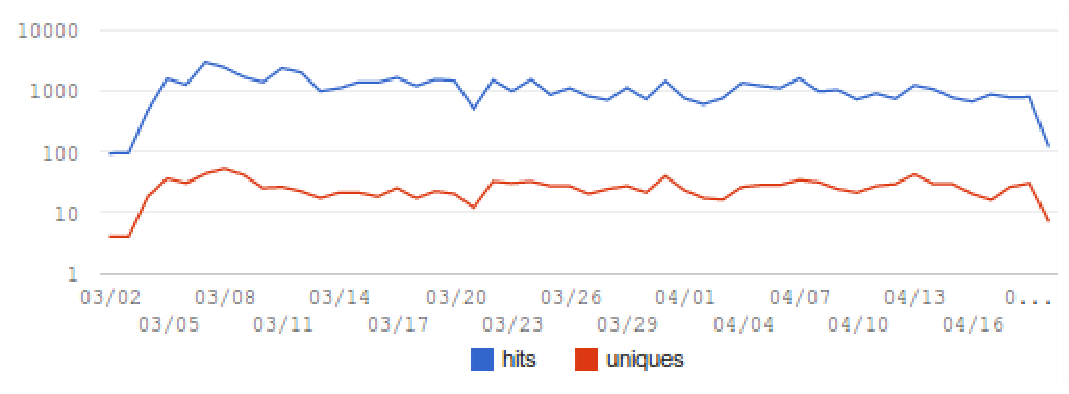
\includegraphics[width=13.45cm]{img/ud_active_users.pdf}
	\caption{Aktivita uživatelů Chum.ly.}
	\label{img:chumly_active_users}
\end{figure}


Na obrázku \ref{img:chumly_active_users} je znázorněn denní počty uživatelů Chum.ly (červeně) spolu s počtem kliků za jednotlivé dny (modře). Chum.ly má v průměrně třicet aktivních uživatelů denně, kteří dohromady udělají tisíc kliků. Tento základní údaj je zobrazen pro všechny skupiny - návštěvníky, registrované uživatele a platící uživatele.  



\begin{figure}[h]
	\centering
	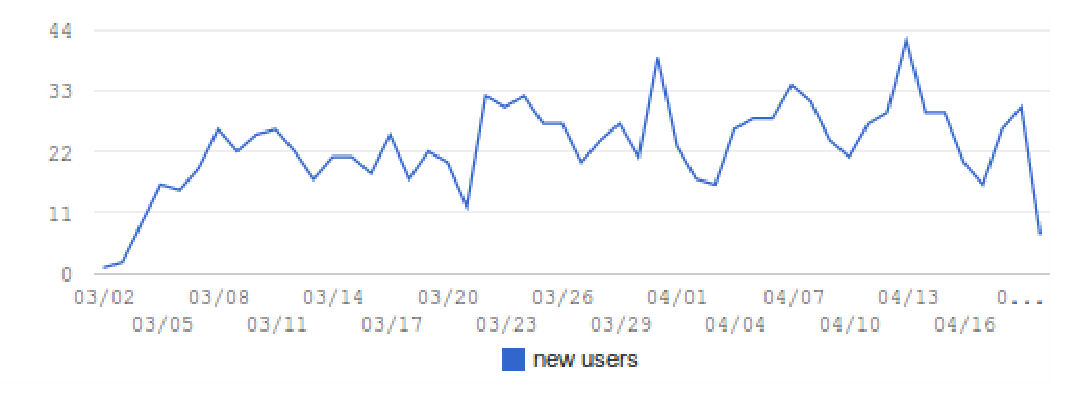
\includegraphics[width=13.45cm]{img/ud_new_users.pdf}
	\caption{Noví uživatelé Chum.ly}
	\label{img:chumly_new_users}
\end{figure}

Pro tento graf a některé další jsem vybral logaritmické měřítko. Jelikož jsou grafu zobrazeny veličiny s řádovým rozdílem je na něm lépe vidět porovnání obou křivek.

Na graf aktivních uživatelů navazuje znázornění počtu akvizice nových uživatelů (obr \ref{img:chumly_new_users}). Podobný graf je zobrazen na všech kartách, takže uživatel vidí jaký má nárůst návštěvníků, uživatelů a platících zákazníků. Rozhraní aplikace je psané v angličtině a proto jsou i data na obou grafech ve formátu měsíc/den. 


Tyto dva grafy představují základní přehled o používání aplikace a akvizici nových uživatelů. Každý provozovatel webové aplikace by tyto grafy měl mít každý den na očích, aby přel představu o svém byznysu. Pokud počet nových uživatelů je nulový, nebo počet aktivních uživatelů nestoupá, je třeba nějak zakročit. To stejné platí pro platící uživatele, jejich počet by měl stoupat a počet nových platících uživatelů by měl být přinejmenším vyrovnaný s počtem platících uživatelů, kteří aplikaci opouští.

Z hlediska porovnání s dostupnými nástroji a tím, co si může výrobce webové aplikace naprogramovat sám může každý provozovat webové aplikace zjistit kolik má v daném okamžiku uživatelů, nebo použít Google Analytics. Pokud to chce znát počet aktivních uživatelů, zákazníků a návštěvníků, musí v si to umět nastavit a vědět, které statistiky sledovat. Jelikož však Google Analytics nepracuje s jednotlivými uživateli, není již možné získat detailní informace o jednotlivých uživatelích.

S mým produktem jakékoli konfigurace a nastavování odpadá a výsledky jsou vyextrahovány z dostupných informací o zákazníkovi. Přesto, že se do měřícího skriptu zadává pouze několik údajů, je možno z nich získat široké spektrum informací. Tím, že se produkt zabývá pouze měřením webových aplikací dokáže poskytnout sadu statistik, které provozovatelé potřebují, bez nutnosti zdlouhavé konfigurace.

Na obrázku \ref{img:users_table} je tabulka znázorňující seznam nedávných uživatelů aplikace a nejaktivnějších uživatelů. Tato relativně jednoduchá funkcionalita již překračuje možnosti drtivé většiny nástrojů pro měření webových stránek. 


\begin{figure}[h]
	\centering
	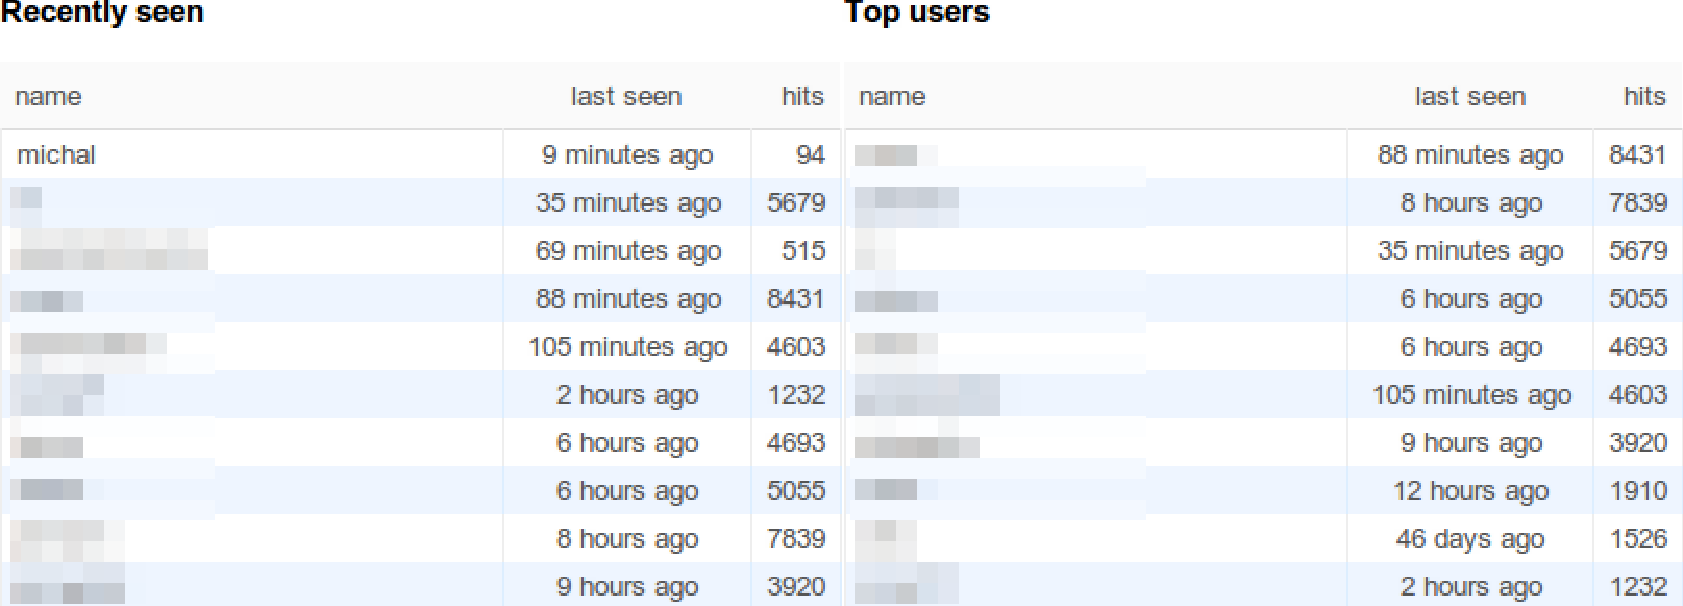
\includegraphics[width=15cm]{img/users_table.pdf}
	\caption{Z leva: nedávno vidění a nejaktivnější uživatelé.}
	\label{img:users_table}
\end{figure}

Tyto informace mají mnoho využití. Například našel jsem uživatele, který byl na chum.ly velmi aktivní a najednou přestal chodit. Vžil jsem se do role majitele webové aplikace a šel zjistit, co se stalo. Ukázalo se, že před čtyřiceti šesti dny zlomil nohu a byl v nemocnici bez internetu. 

Kdyby se jednalo o platícího zákazníka, pomohla by mi tato informace v rozhodování, zda mu účet zamrazit, nebo smazat. Je tedy možno zaujmout více individuální přístup k zákazníkům, kteří to pravděpodobně ocení a mohou pak z vlastní pozitivní zkušenosti aplikaci doporučit.

Po kliknutí na jméno v tabulce se zobrazí detailní přehled uživatele (obrázek \ref{img:user_profile}). Je z něj vidět, zda se jedná o platícího zákazníka, nebo uživatele (položka "Class"). Pro případ nutnosti kontaktu jeho email, kdy byl naposledy vidět a kdy byl poprvé zaznamenán. Napravo od profilu je graf s počtem kliknutí v jednotlivých dnech.

\begin{figure}[h]
	\centering
	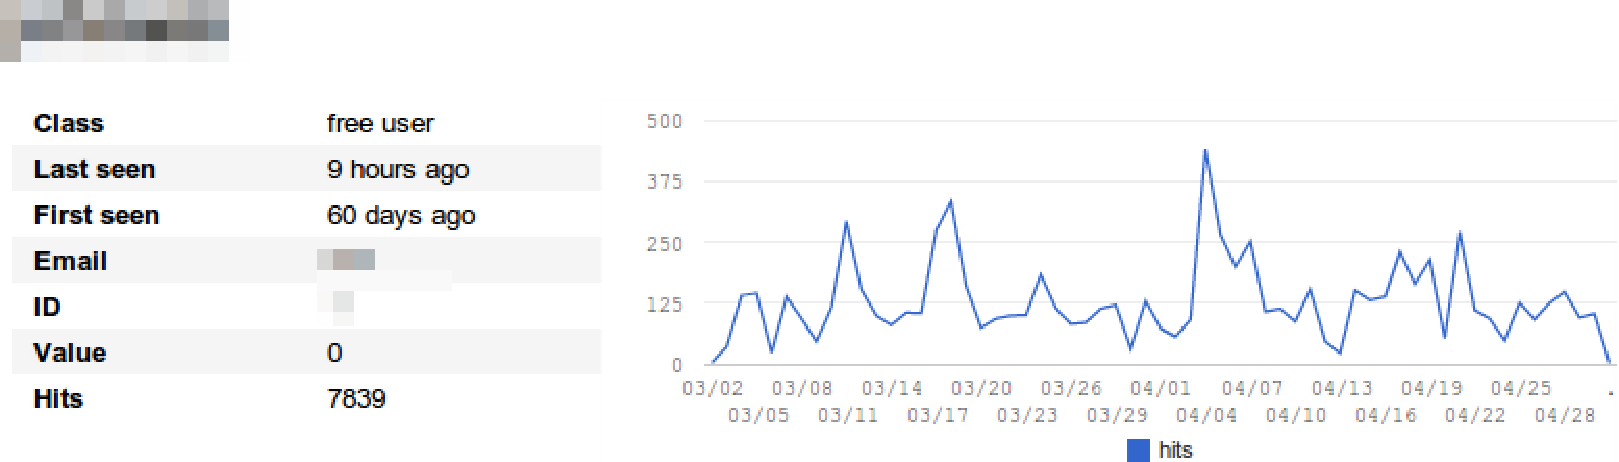
\includegraphics[width=15cm]{img/user_profile.pdf}
	\caption{Profil uživatele.}
	\label{img:user_profile}
\end{figure}

Na obrázcích \ref{img:chumly_features} a \ref{img:chumly_features_nolog} je znázorněna absolutní používanost jednotlivých funkcí v čase. Prvním graf používá logaritmické měřítko, druhý lineární. V tomto případě se mají obě zobrazení svoje pro a proti. 

Předpokládám, že u aplikace s řádově vyšším počtem uživatelů by logaritmický graf zobrazoval vyrovnanější křivky. Ne každá aplikace však bude mít tisíce uživatelů denně, takže v tomto případě a podobných bude třeba nabídnout přepnutí měřítka grafu a případně přiblížení nebo další pohledy.


\begin{figure}[h]
	\centering
	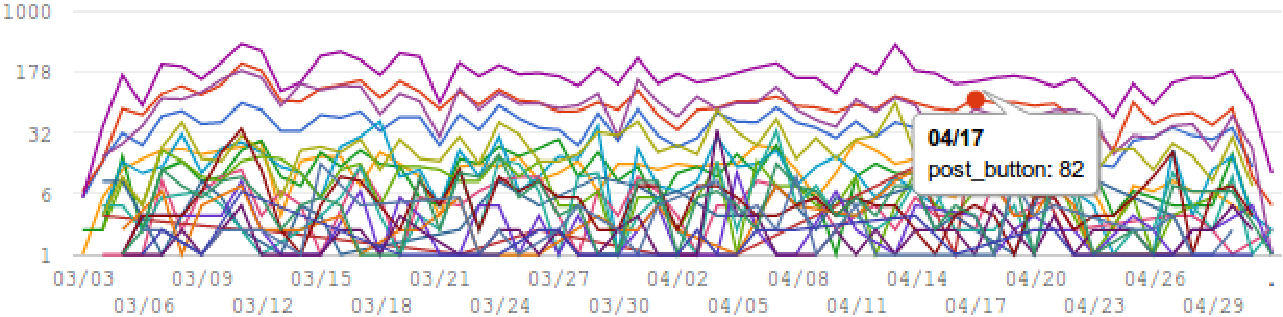
\includegraphics[width=15cm]{img/chumly_features_small_nolegend.pdf}
	\caption{Četnost používání jednotlivých funkcí v logaritmickém měřítku}
	\label{img:chumly_features}
\end{figure}


\begin{figure}[h]
	\centering
	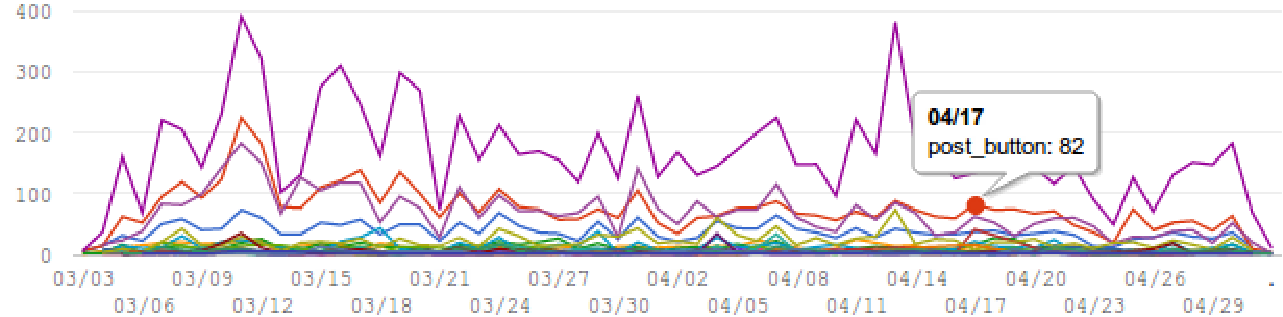
\includegraphics[width=15cm]{img/chumly_features_small_nolog_nolegend.pdf}
	\caption{Četnost používání jednotlivých funkcí v lineárním měřítku}
	\label{img:chumly_features_nolog}
\end{figure}

Známé funkce sledované aplikace také umožňují identifikovat akce provedené u\-ži\-va\-te\-lem. Jednotlivé akce, které uživatel dělá se pak shlukují do jednotlivých návštěv. Jelikož výpisy návštěv obsahují informace o tom, co uživatel zhruba dělal, říkám jim příběhy.

\begin{figure}[h]
	\centering
	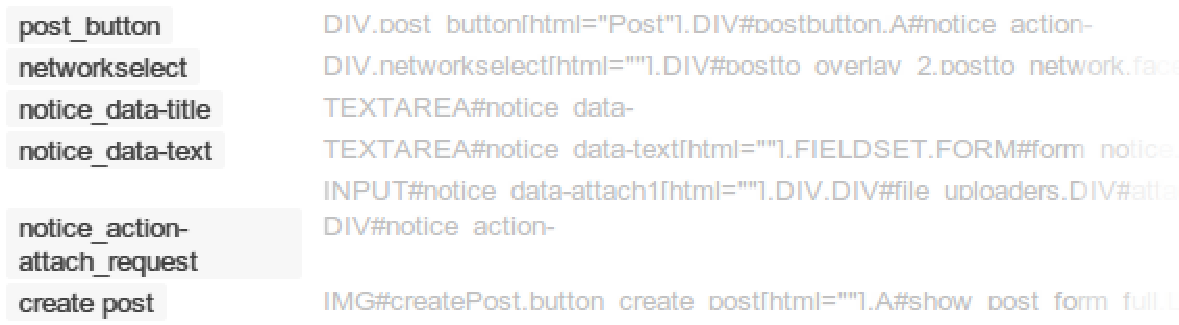
\includegraphics[width=14.65cm]{img/user_story.pdf}
	\caption{Jeden příběh, jedná se o vytvoření zprávy.}
	\label{img:user_story}
\end{figure}


Na obrázku \ref{img:user_story} je vidět takovýto jeden příběh. Uživatel kliknul na tlačítko, které otevře formulář s vytvořením nové zprávy. Poté nastavil, do které sociální sítě chce zprávu poslat, vepsal titulek zprávy a text. V dalším okamžiku připojil přílohu (obrázek, zvuk, nebo jiný soubor) a potvrdil vytvoření zprávy.

Jednotlivé funkce aplikace jsou definovány pomocí jednoduchého rozhraní, ve kterém uživatel "nakliká" funkce, které má zájem sledovat (obrázek \ref{img:define_features}). Vytvořené funkce jsou automaticky pojmenovány podle pozice v struktuře dokumentu a sémantiky a uživatel má možnost názvy změnit.

\begin{figure}[h]
	\centering
	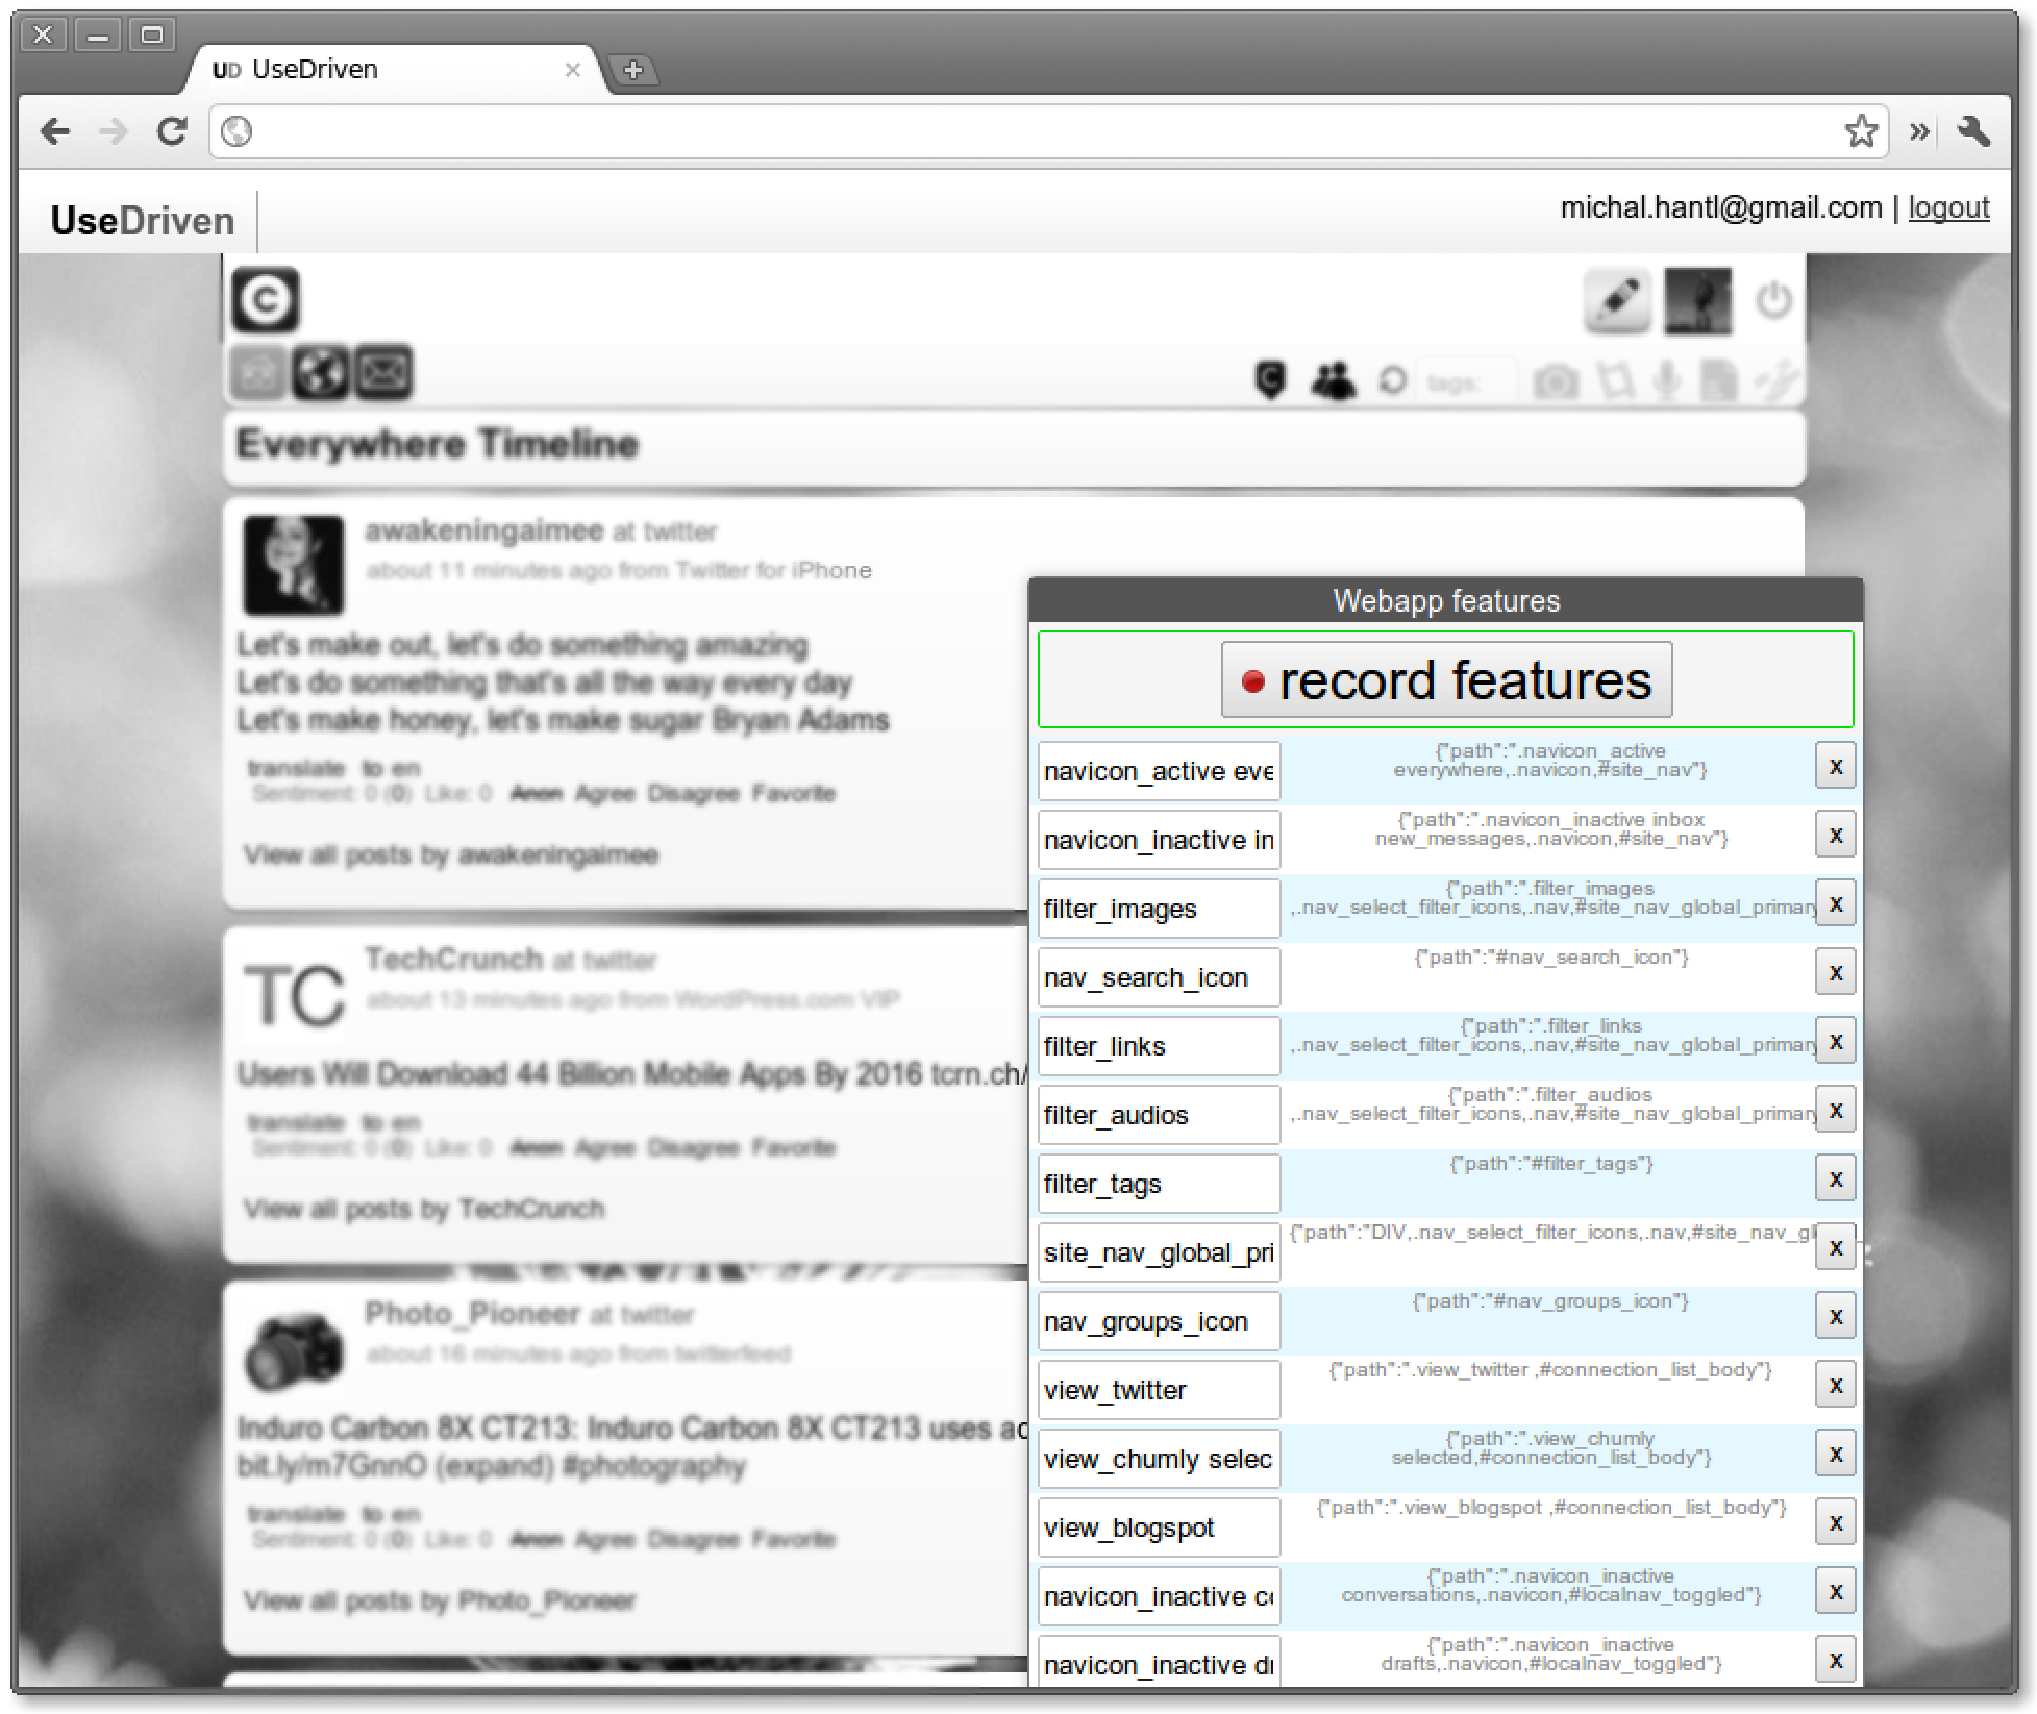
\includegraphics[width=14cm]{img/ud_chumly_define_features_blurry_bw.pdf}
	\caption{Definování sledovaných funkcí pomocí grafického rozhraní}
	\label{img:define_features}
\end{figure}

Mimo jiné obsahuje aplikace i nástroje pro vývojáře, které generují náhodné data, jsou schopné importovat a exportovat data a spravovat metriky. Na obrázku \ref{img:developer_features} jsou jednotlivé metriky a jejich aktuální stav. V případě, že se nějaká metrika "zasekne", je možno ji odblokovat, případně promazat data nebo zcela metriku odebrat.

Každá metrika je schopna sekvenčním procházením zpracovávat události měřené aplikace a produkovat výstup v normovaném tvaru, který je zobrazován na grafech. Do budoucna je možné nechat uživatele vytvářet vlastní grafy, ve kterých se promítnou metriky, které si uživatel zvolí pomocí grafického uživatelského rozhraní.

\begin{figure}[h]
	\centering
	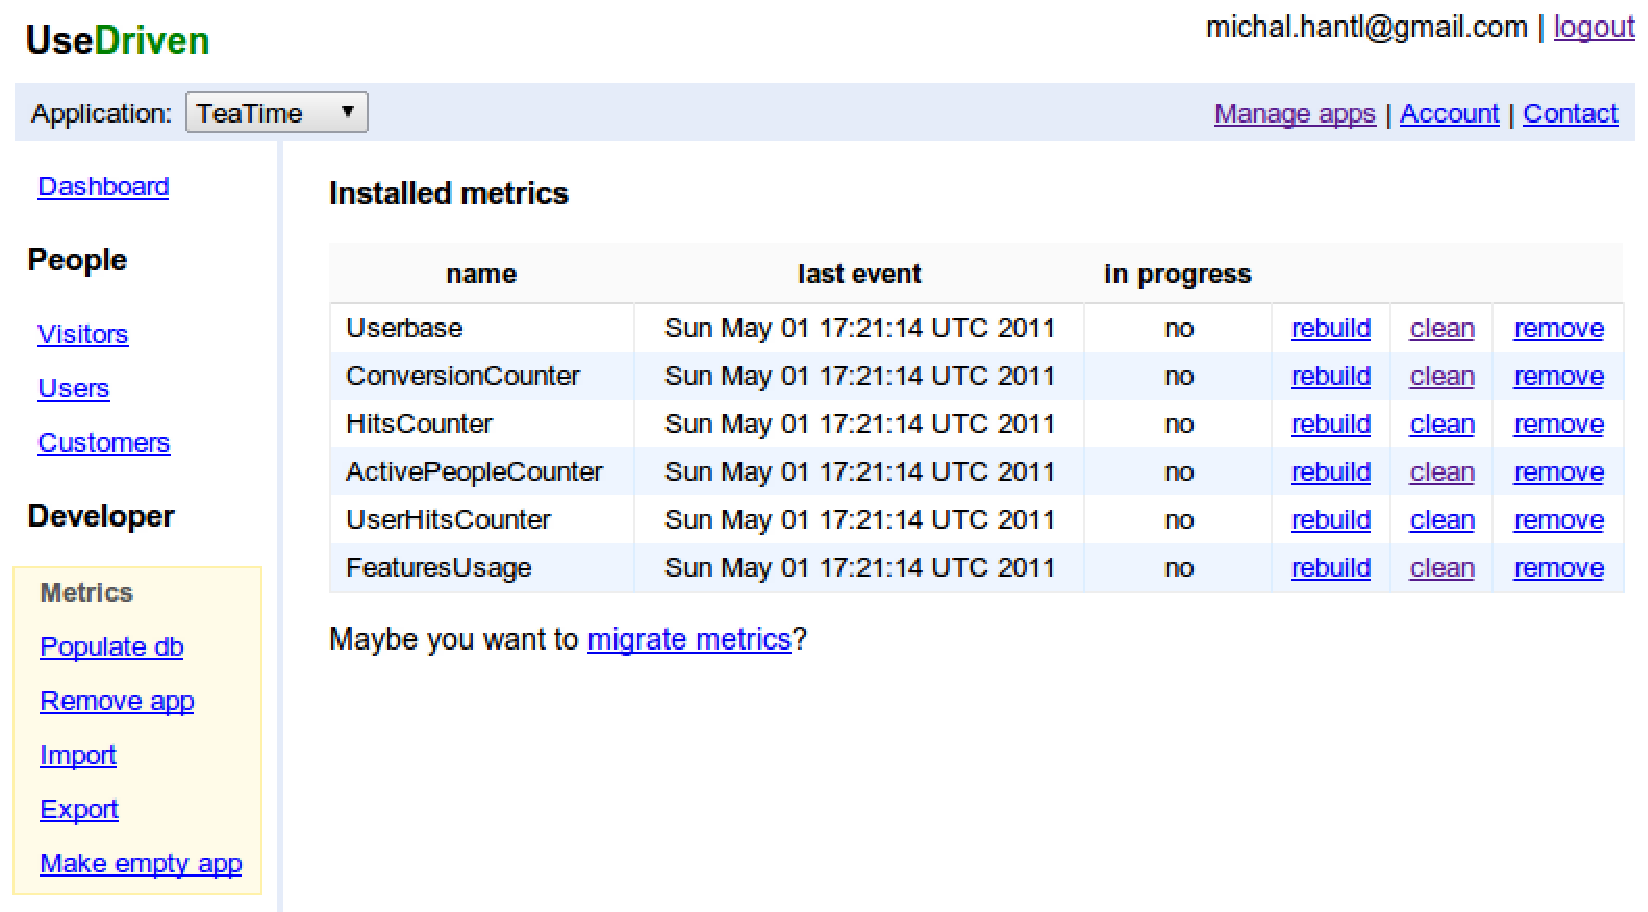
\includegraphics[width=14.65cm]{img/developer_functions.pdf}
	\caption{Celé rozhraní aplikace. Karta funkce pro vývojáře.}
	\label{img:developer_features}
\end{figure}

V neposlední řadě aplikace obsahuje kontaktní formulář, který odesílá email tvůrci, úpravu uživatelského účtu a podporu více aplikací pro jednoho uživatele. Během vývoje aplikace jsem se snažil zohlednit potřeby uživatele i správce aplikace tak, že jsem trávil více času na funkcích, které byly používány častěji.








\subsection{Zhodnocení}

Na závěr jsem požádal představitele Chum.ly o názor na vyvinutý nástroj. Zajímalo mě, jak se jim jeví vzhledem k praktické využitelnosti pro jejich webovou aplikaci, co konkrétně je zaujalo a jaký je rozdíl mezi jinými nástroji, které používají.

Aplikaci jsem prezentoval technickému řediteli Chum.ly Marcu Quinlivanovi\footnote{Marc Quinlivan \url{http://ie.linkedin.com/in/quinlivanmarc}}, který ji již předtím používal a toto je jeho vyjádření.

\begin{quote}
UseDriven has provided us with some very useful statistics about our
service. It allows us to trend our user loyalty and track returning visits. We can also see which users are most active and which users have not
returned in a while. This allows us to identify users and contact them to better understand the reasons why they are no longer active.

With the feature tracker we can see which buttons or features are being used most and which ones are not being used at all. This can assist with our site design as we can move more popular features to a better position, remove unused features, or possibly move those less used features to a location where they will be more visible to try to generate more use.

With UseDriven we are able to gain more in-depth details about our users and visitors than is possible with similar services, such as Google
Analytics.
\end{quote}

Uvádím také volný překlad do češtiny.

\begin{quote}
UseDriven nám poskytl některé velmi užitečné statistiky o naší službě. U\-mo\-žňu\-je nám sledovat trend naší uživatelské loajality a sledovat vracející se návštěvy. Můžeme také vidět, kteří uživatelé jsou nejaktivnější, a kteří se dlouho neukázali. To nám umožňuje identifikovat odcházející uživatele, spojit se s nimi a lépe pochopit důvody, proč již nejsou aktivní.

Pomocí sledování četnosti používání funkcí vidíme, která tlačítka a funkce jsou používány nejvíce a které nejsou používány vůbec. To může pomoci s designem našeho situ, může posunout populárnější funkce pro na lepší pozice a odstranit nepoužívané funkce, případně přesunout ty méně používané funkce do místa, kde budou více vidět, abychom se pokusili zvýšit jejich používanost.

Pomocí UseDriven jsme schopni získat více hloubkové informace o našich uživatelích a návštěvnících, než je možné s podobnými službami, jako jsou Google Analytics.
\end{quote}

\begin{comment}
\subsubsection{Budoucí vývoj a uplatnění}

Nebudu navrhovat změny pro chum.ly, ale změny nástroje.

 - trackovat referrery
 - 



Globální pohled
 - jak dlouho jsem nad tím strávil
 - co jsem mezitím organizoval? :)
 - zmínit, že jsme v kanclu

O Mirah a AppEnginu
 - očekávání
 - co to přináší (Google Datastore, škálovatelnost, cloud, rozvoj platformy)
 - co to stojí.

O nástroji
  - jaké bylo očekávání
  - jeho využitelnost v praxi a přínos pro provozovatele webových aplikací.
  - porovnání s podobnými nástroji
  
O procesu
  - co jsem se naučil
  	- mirah, appengine, time management
  - co bych dělal jinak
  	- dobrá otázka
  - co bych dělal stejně
  	- appengine
  - co mě překvapilo 
  	- jak si urovnám psaní myšlenky
  
Jak se změnil můj pohled na vývoj aplikací?
\end{comment}


\section{Závěr}
\label{sec:Conclusion}








\begin{comment}
Vyjít ze zadání...

Cílem práce je vytvoření nástroje, jakožto podpory pro aplikaci a navržení metody získávání informací o chování uživatele webové aplikace. Nebude se jednat pouze o klasický přístup založený na sběru statistických dat anonymních návštěvníků, ale o využití znalosti o konkrétním uživateli, jeho chování, využívání funkcí a služeb webové aplikace.

1. Zanalyzujte a popište možnosti monitorování chování návštěvníků webových stránek a aplikací, a to s důrazem na získané informace a metody jejich zpracování.
2. Navrhněte a popište technické postupy a metody pro získávání potřebných informací a dat o chování uživatele.
3. Naimplementujte nástroj pro monitorování chování návštěvníků webových aplikací, a to včetně modulu pro integraci do jakékoli webové (HTML) aplikace.
4.Vyvinutý nástroj aplikujte do provozu a získaná data analyzujte a popište závěry plynoucí ze získaných informací.
5.Zhodnoťte vyvinutý nástroj především z pohledu reálného nasazení a jeho přínosů, porovnejte jej s obdobnými nástroji a jejich metodami.
\end{comment}

% čo som mal spraviť

Cílem práce bylo vytvořit nástroj pro podporu webových aplikací a navržení metody měření chování jejích uživatelů při využití znalosti konkrétního uživatele, jeho chování a využívaných funkcí webové aplikace.

% čo som spravil, čo som nespravil

Vytvořil jsem metodu i nástroj, který umožňuje snadno měřit webové aplikace pomocí měřícího vložení skiptu do zákaznické aplikace. Nástroj byl vyvinut pro platformu Google AppEngine v jazyce Mirah a tam byl také nasazen.  Potenciální zákazník, se kterým jsem měl v minulosti dobrý vztah mi umožnil nástroj nasadit na jeho webové aplikaci a měřit ji. Vytvořil jsem abstrakci pro zpracování měřených dat, které mi umožňuje do\-pl\-ňo\-vat nové interpretace a prezentoval jsem výsledky měření.

% výhľady do budůcna

Tuto aplikaci jsem vyvinul se záměrem prorazit na americký trh s vlastním produktem pro podporu webových aplikací. Budu pokračovat v jejím vývoji s klíčovými zá\-ka\-zní\-ky a v horizontu několika měsíců chci začít s monetizací.










\begin{comment}
\bigskip
\begin{flushright}
Michal Hantl
\end{flushright}
\end{comment}


\section{Přílohy}

\begin{enumerate}
\item \textbf{Kompaktní disk} obsahující elektronickou verze dokumentu, zdrojové kódy a návod k instalaci.
%TODO doplnit strukturu CD
\end{enumerate}







\begin{thebibliography}{99}


\bibitem{kaushik} Kaushik, Avinash
\textit{Web Analytics 2.0}, Sybex, 2009. ISBN 9780470529393.

%\bibitem{kaushik} Kawasaki, Guy
%\textit{The Art of the Start}, Portfolio Hardcover, 2004. ISBN 9781591840565.

\bibitem{webgl} Chris Marrin,
\textit{WebGL Specification}, dostupné z url \url{https://www.khronos.org/registry/webgl/specs/1.0/}.

\bibitem{browser_market_share} w3schools,
\textit{Browser Statistics}, dostupné z url \url{http://www.w3schools.com/browsers/browsers_stats.asp}.


\bibitem{urchin} New York Times,
\textit{Google Acquires Urchin Software}, dostupné z url \url{www.nytimes.com/2005/03/29/technology/29urchin.html}.

\bibitem{clf} W3C,
\textit{Common logfile format}, dostupné z url \url{www.w3.org/Daemon/User/Config/Logging.html#common-logfile-format}.


\bibitem{url} Network Working Group,
\textit{Uniform Resource Locators}, dostupné z url \url{www.ietf.org/rfc/rfc1738.txt}.

\bibitem{heatmap} Business Insider,
\textit{Bing Is Better For Ads Than Google}, dostupné z url \url{www.businessinsider.com/microsoft-bing-has-a-more-ad-} \url{friendly-design-than-google-according-to-heatmaps-2009-6}.


\bibitem{conversions} Justin Cutroni,
\textit{How Does Google Analytics Track Conversion Referrals?}, dostupné z url \url{http://cutroni.com/blog/2006/11/10/how-does-google-analytics-track-conversion-referals/}.

%\bibitem{gae} Sanderson, Dan
%\textit{Programming Google App Engine}, O'Reilly Media, 2009. ISBN 059652272X.


%Článek o akvizici v New York Times \url{http://www.nytimes.com/2005/03/29/technology/29urchin.html}


\bibitem{cdn} Björn Sållarp,
\textit{Google App Engine as your CDN?}, dostupné z url \url{http://blog.sallarp.com/google-app-engine-cdn/}.


\bibitem{visitor} Dvořák, Miloš,
\textit{Visitor Pattern}, dostupné z url \url{http://objekty.vse.cz/Objekty/Vzory-Visitor}


\bibitem{cookies} Jak Psát Web,
\textit{Cookies}, dostupné z url \url{www.jakpsatweb.cz/enc/cookies.html}.

\bibitem{bigtable} Google Research Publications,
\textit{Bigtable: A Distributed Storage System for Structured Data}, dostupné z url \url{http://labs.google.com/papers/bigtable.html}.


\bibitem{chart_tools} Google,
\textit{Google Chart Tools}, dostupné z url \url{http://code.google.com/apis/visualization/documentation/using_overview.html}.

\bibitem{billing} Google AppEngine,
\textit{Billing and Budgeting Resources}, dostupné z url \url{http://code.google.com/appengine/docs/billing.html}.





\end{thebibliography}


%\appendix
%\section{Grafy a měření}
%Tohle je příloha k práci. Většinou se sem dávají grafy, tabulky, které by vzhledem
%ke svému počtu překážely v textu diplomky.
%\clearpage




\end{document}